\chapter{Architecture}
\label{chap:architecture}

Crowdsourcing based on simple, independent and deskilled list of tasks basically 
limits the scope and complexity of problems can be tackled. Independent tasks that 
are narrowly focused and low-complex cannot be easily utilized to solve complex 
problems. Although simplicity and interdependency enable easily distributed and 
parallelized processing, complex and sophisticated problems require efficient and 
effective coordination in which problem itself is the decomposed into multiple stages. 
Each stage requires allocation of appropriate resources, in addition to the management of interdependencies among stages.

The need for new powerful programming paradigm that can handle the advanced 
problem-solving is clearly stated~\cite{Doan2011, Kittur2013, Bernstein2012}. 
The new paradigm or framework is required to be able to 
\begin{itemize}
	\item tackle advanced problems with no rigid limitations
	\item decompose problems into smaller pieces (or tasks)
	\item manage dependencies among different tasks
	\item allocate appropriate resources to each task
	\item reflect the skill-set of people and computers while solving tasks.
\end{itemize}

$Crowdy$ is an extensible, general-purpose crowdsourcing platform to solve 
complex problems. The platform is developed over the fundamentals of stream 
processing paradigm for which a series of operations are applied to the continuous 
stream of data elements via operators~\cite{Gedik2014}.

$Crowdy$ is an operator-centric platform. Using this platform, a requester with no 
requirement of a programming background can quickly translate a complex problem into 
a crowdsourcing application by simply selecting operators and connecting these operators 
together. As a result of $Crowdy$'s focus on operators, requesters can design applications 
by selecting right set of building blocks that are necessary to solve their problem, 
and customizing these blocks particular to the computation to-be-conducted.

$Crowdy$ embodies several features:
\begin{itemize}
	\item A standard toolkit of operators that can both human and software resources 
	(human or software) to accomplish various tasks
	\item Configuration support to control and coordinate resource utilization 
	\item Customizable collaborations over parameterization
	\item Application runtime interface
\end{itemize}

\section{Architecture using Component-and-Connector Views}


$Crowdy$ platform is implemented as a REST~\cite{Richardson2008} architecture. 
Applications are developed, configured and validated on the client-side. These 
applications are submitted to server-side via an application programming interface 
(API) over HTTP. The execution happens on the server-side and results are kept 
in a database server.

In the following, the architecture design is explained using Views and Beyond approach
~\cite{Clements}. Views and Beyond approach is useful for identification and documentation of 
design decisions made. Component-and-connector (C\&C) views are used to document 
presence of runtime elements and their interactions.

Figure~\ref{fig:arch} illustrates the primary presentation of the system's 
runtime architecture. It is showing a picture of the system as it appears at runtime. 
A set of clients can interact with the application server, embodying a client-server 
style. The client components communicate with application server components 
via the API defined by the server. Client components can achieve a set of operations 
such as creating a new application, getting results for an existing application over that API.

The system contains a shared repository of $tasks$ in \textit{database server} 
accessed by the application server. The $task$ database is the list of action 
items per application. New tasks can be created for new applications or a 
list of uncompleted tasks can be completed 
with an API call from the application server. Thus, the connection between the 
application server and the task database is handled by API as well.

The system has another server that is \textit{crowdsourcing platform server}. This 
server provides the required resources for human computation. The resource 
allocation and usage using this component are handled by HTTP API calls too. 
The application server does the API calls.

%\begin{figure}[ht]
%	\centering
%	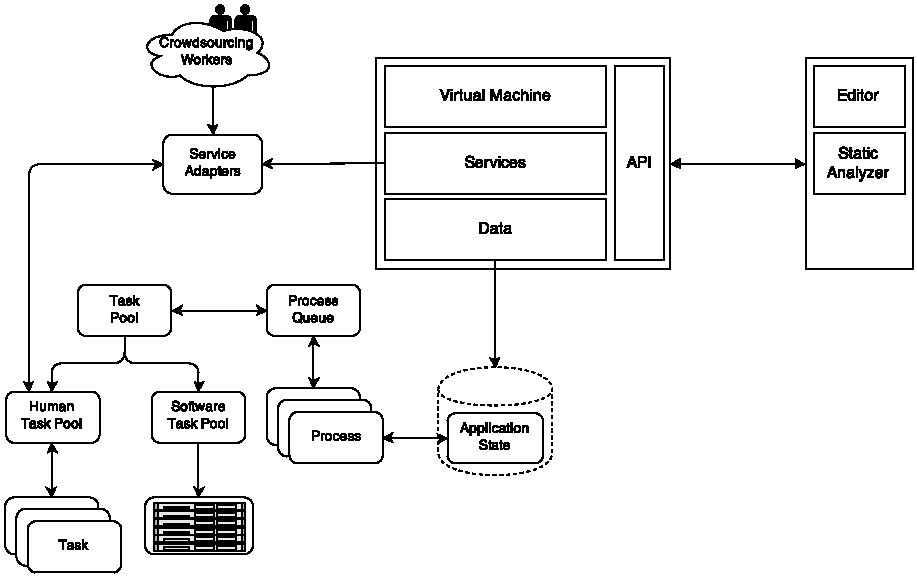
\includegraphics[height=200px]{figures/Architecture.pdf}
%	\caption{Architecture of the platform.}
%	\label{fig:architecture}
%\end{figure}

\begin{figure}[ht]
	\centering
	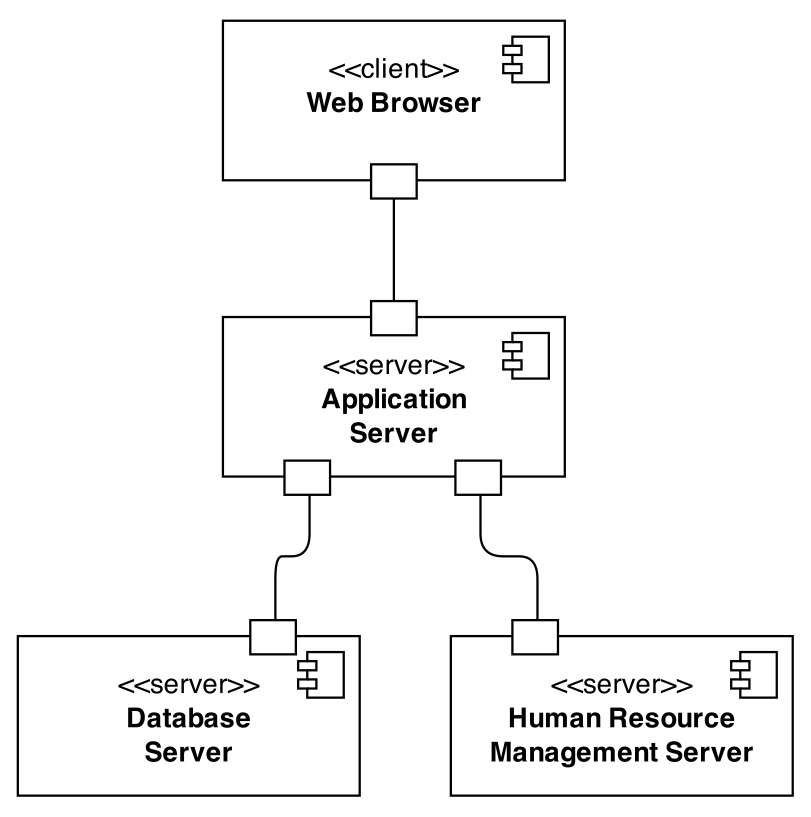
\includegraphics[width=0.6\textwidth]{figures/architecture/CC1.png}
	\caption{Architecture of the platform.}
	\label{fig:arch}
\end{figure}

The client-side of $Crowdy$ is where crowdsourcing applications are developed. Client 
part consists of two components: \textit{workflow editor} and \textit{static analyzer}. The 
\textit{workflow editor} sits on top of \textit{static analyzer} as shown in Figure
~\ref{fig:clientdecomposition} and uses it's services to analyze applications.

\begin{figure}[ht]
	\centering
	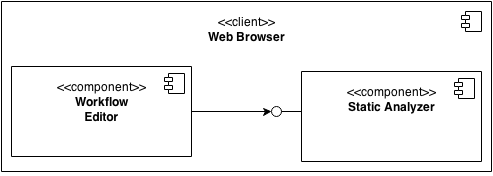
\includegraphics[width=0.5\textwidth]{figures/architecture/CC2.png}
	\caption{Logical decomposition of client-side architecture.}
	\label{fig:clientdecomposition}
\end{figure}

The \textit{workflow editor} is where applications are designed. The editor provides 
users a list of available operators and a flow composition panel. An application is 
a flow where information flows from source to sink operators. An operator can be 
created by dragging from the list to the flow composition panel. A flow is created by 
connecting one operator to another.

The \textit{static analyzer} runs all the time during the application development. This 
component checks the validity of the application. Warnings and errors are raised 
when user tries an action that can result in an invalid application. When user is 
ready to submit application to the server-side for execution, \textit{static analyzer} 
does a final validation check. If validation succeeds, application can be submitted 
to the server-side and execution can be started.

The server-side of $Crowdy$ is where crowdsourcing applications are executed and 
results are generated. Server part consists of three components: \textit{API}, 
\textit{virtual machine} and \textit{service adapters}. In addition, server-side 
is connected a database server and a crowdsourcing platform server. 
Figure~\ref{fig:serverdecomposition} demonstrates the logical decomposition of these 
components and their usage relation.

\begin{figure}[ht]
	\centering
	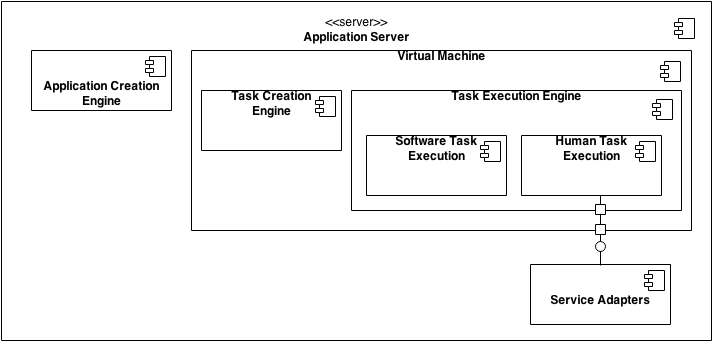
\includegraphics[width=0.85\textwidth]{figures/architecture/CC3.png}
	\caption{Logical decomposition of server-side architecture.}
	\label{fig:serverdecomposition}
\end{figure}

The \textit{application programming interface (API)} on the application server 
specifies how client-side should interact with server-side. Client-side submits 
application and receives the details of an application state via \textit{API} using 
remote HTTP calls. \textit{API} creates and updates applications. Application 
states are saved into \textit{database server}.

The \textit{virtual machine} is a component responsible for executing applications. 
It provides service-independent environment for human computations. The 
\textit{database server} is periodically checked, processes are created, and 
required computation resources are allocated by \textit{virtual machine}. These 
processes are then executed and results are saved again into \textit{database server}. 
\textit{Virtual machine} uses the server itself to execute processes that needs 
software resources. The \textit{service adapters} component is utilized to allocate 
human resources.

The \textit{service adapters} component provides an interface to \textit{virtual machine} 
to execute processes that require human computation. This component uses and 
adapts \textit{API}s provided by external crowdsourcing platform servers. The requests 
from \textit{virtual machine} are translated into requests that external APIs can 
understand and submitted there. After process completion, results are gathered and 
saved into \textit{database server}.

The \textit{database server} is where application state is kept. It is accessed by 
\textit{API} and \textit{virtual machine} to create new applications and update 
application state correspondingly.

Figure \ref{fig:componentconnector} demonstrates the architecture via components 
and connectors. As explained before this is an client-server architecture in which 
the connections in between web services are handled by APIs over HTTP. 
Considering architecture from this perspective reveals the significance of 
\textit{virtual machine} within \textit{application server}. \textit{Virtual machine} 
connected to \textit{database server} and \textit{service adapters} constitutes 
the idea of stream-based human computation.

\begin{figure}[ht]
	\centering
	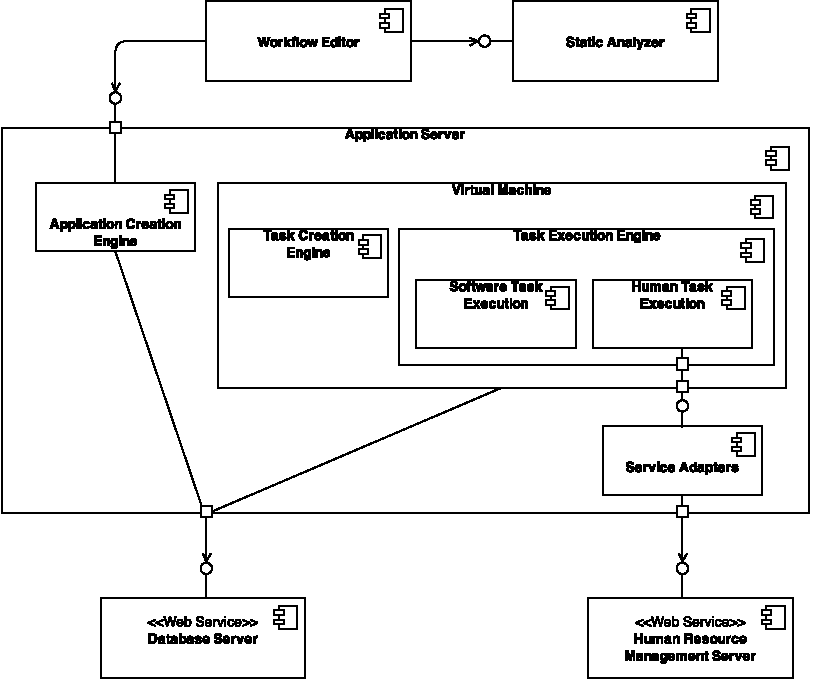
\includegraphics[width=0.85\textwidth]{figures/architecture/ComponentConnector.pdf}
	\caption{Architecture in terms of components and connectors.}
	\label{fig:componentconnector}
\end{figure}

Applications created by \textit{application creation engine} via the submissions from 
\textit{workflow editor} are saved into \textit{database server}. As mentioned before 
\textit{virtual machine} periodically checks \textit{database server}, and either 
creates new tasks or executes the existing ones. In that sense, \textit{virtual machine} 
has two basic components: \textit{task creation engine} and 
\textit{task execution engine}. \textit{Task creation engine} retrieves newly submitted 
applications and creates the initial task, which conforms to jobs of 
\textit{source operator} (see concept explanations later in the chapter). Task created 
by \textit{task creation engine} is saved back to the database with the information 
required for task execution. \textit{Task execution engine} receives the available 
tasks from \textit{database server}. The task is tagged as software-related or 
human-related based on the details. If task is software-related such as saving 
a text into a file or sending an email, then it is executed by 
\textit{software task execution} component. Otherwise, task is human-related and 
that means this specific task requires human resources. Therefore, task 
is received by \textit{human task execution} component. This component decides 
the necessary resources for execution and allocates them via \textit{service adapters} 
component, which accesses \textit{human resource management server} via it's API. 
Task is then executed by human workers and results are sent back from 
\textit{human resource management server} to \textit{human task execution} 
component via \textit{service adapters}.

In the remainder, the fundamental concepts of $Crowdy$ are explained 
in more detail and features are explored as we look into various aspects of application 
development using $Crowdy$ platform. In Section~\ref{sec:tool} the tool developed over 
these concepts is explained, and a sample application is developed using the tool.




\chapter{Platform}
\label{chap:platform}
$Crowdy$ applications are developed to solve complex and sophisticated problems 
that require both human intelligence and computing power. A typical application contains 
three main high-level components: data ingest, processing and data egress.

\begin{figure}[ht]
	\centering
	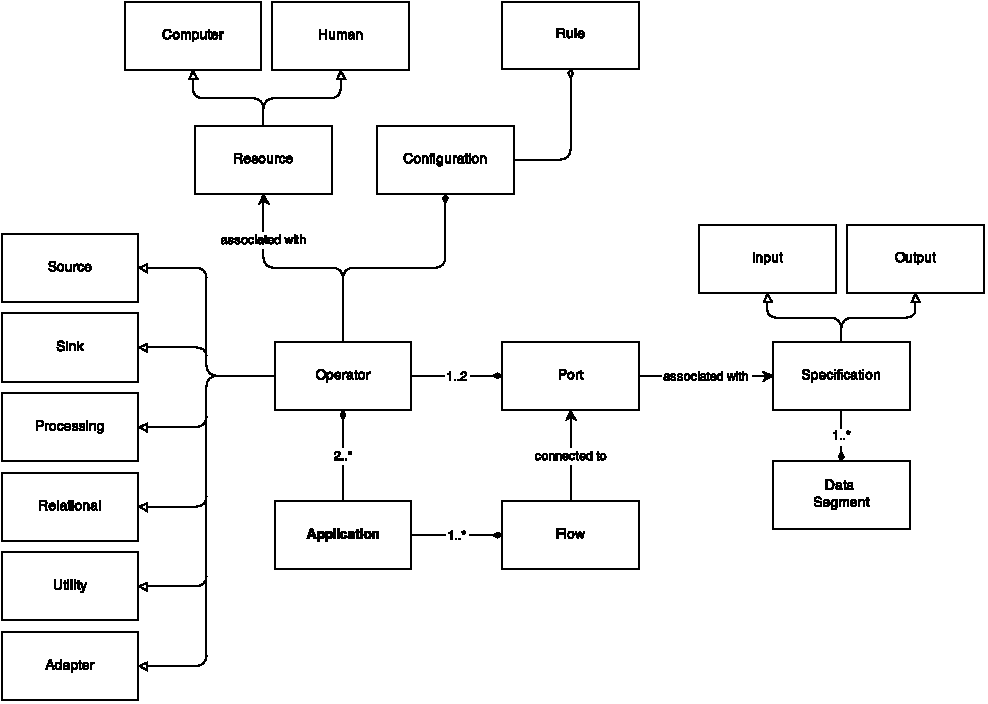
\includegraphics[width=0.9\textwidth]{figures/ApplicationMetamodel.pdf}
	\caption{Metamodel for a Crowdy application.}
	\label{fig:metamodel}
\end{figure}

Figure~\ref{fig:metamodel} shows the metamodel for which a $Crowdy$ application is 
based on. An application is formed by a set of \textit{operator}s. As mentioned before, 
typically an application has three \textit{operator}s: one for inputting data, one for processing 
that data items, and finally one for outputting the results. However, it is possible to 
have an application with only two \textit{operator}s: one for data input and other for data 
output.

Each \textit{operator} is associated with a type that can be one of \textit{source, sink, 
processing, relational, utility, adapter}. Based on it's type, operator may have 
one or two \textit{port}s. The number of \textit{port}s is basically decided by the type. 
For instance, \textit{source} and \textit{sink} \textit{operator}s have only one \textit{port}, 
but others have two \textit{port}s. A \textit{port} is associated with a \textit{specification}, 
which can be either \textit{input} or \textit{output} \textit{specification} again based on 
it's type. \textit{Specification} is formed by \textit{data segment}s that are used to 
convey information through \textit{flow}s. This means \textit{flow}s are the 
components that deliver information from one \textit{operator} to another via \textit{port}s.

\textit{Operator}'s type also determines the type of resource it is associated with. The base 
promise of this study is to combine limited computer and human resources together to 
solve complex problems. Each \textit{operator} is linked to a \textit{resource}, which can be either 
\textit{computer}s or \textit{human}s. While that \textit{operator} is executed, related \textit{resource}s are 
allocated. An \textit{operator} also has \textit{configuration} dependent on it's type. \textit{Configuration} 
may have \textit{rule}s that decide how \textit{operator} will function based on the data.

\begin{figure}[ht]
	\centering
	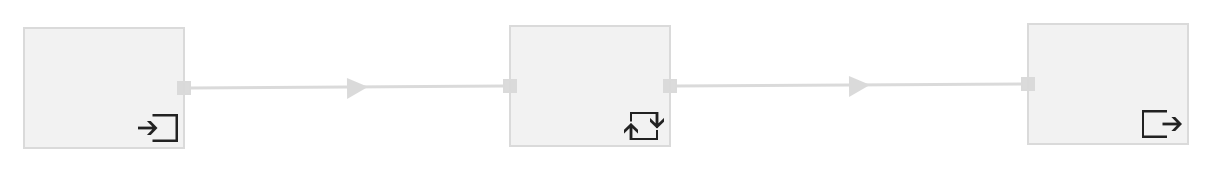
\includegraphics[width=0.85\textwidth]{figures/helloworld.png}
	\caption{A sample, minimal $Crowdy$ application.}
	\label{fig:hello world}
\end{figure}

Let's consider a minimal "Hello World" application that has these three components 
in total, connected in a simple pipeline topology. Figure~\ref{fig:hello world} demonstrates 
the application in the form of a flow graph. On the ingest side, there is a 
\textit{source operator}, which acts like a data generator. Source operator produces 
data tuples that are processed down the flow by the 
\textit{processing operator}. Finally, the \textit{sink operator} simply converts the tuples 
in such a form (text file, email etc) that can be easily interpreted by requesters.

The application flow graph is specified as a series of operator instances and connections 
(data flows) that link them. A data flow basically transfers data tuples 
produced by an operator to another. One or more data segments can be assembled in a 
data tuple via output specification of an operator instance (see Section~\ref{sec:flow comp}). 
In addition, several options can be specified to configure an operator instance. These 
include parameters, operator-specific rules, which are studied in the rest of this chapter.

In a more realistic application, one or more source operators can be employed to produce 
various data tuples that differ in both size and specification. Similarly, the application would 
have one or more processing operators along with other types of operators organized in a way 
that is significantly more complex than this example.

\section{Operator}
\label{sec:operator}
An operator is the basic building block of an application. Operator has a type that is 
specified at the time of creation. This type determines configuration respectively. Also a 
unique ID is assigned to an operator. In addition, operator has optional name and 
description fields that can be used for bookkeeping purposes.

\begin{figure}[ht]
	\centering
	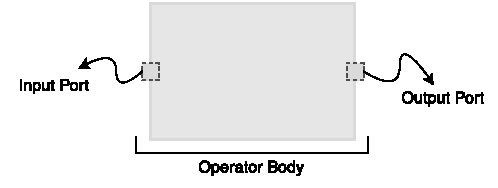
\includegraphics[height=100px]{figures/basicoperator.pdf}
	\caption{Base operator representation.}
	\label{fig:basic operator}
\end{figure}

Operator may have an input port or output port or both corresponding to it's type 
definition. Figure~\ref{fig:basic operator} demonstrates a base operator, which 
consists of a body and ports. Although it is not shown here, each operator presentation 
has a specific icon on their body associated with it's type.

An operator may output tuples to any number of operators, but it can only receive 
tuples from one operator unless it is a union operator (see Section~\ref{sec:utility operators}). 
Union operator can receive tuples from multiple operators and aggregate them,
if these tuples have the same specification. Therefore, consistency of incoming flow 
specification for each operator type is ensured. 
This is a significant feature to guarantee operators functionality, because an operator 
(excluding source operators) uses and operates specifically on the 
information from incoming flow.

$Crowdy$ provides a set of built-in operators that can be used to build applications. 
In general, these operators perform common tasks associated with data generation, 
processing and outputting.

Operators are generally cross-domain to allow general-purpose 
computation possible. They are grouped under six main categories: 
\textit{source, sink, processing, relational, utility, adapter}.

\subsection{Source operators}
The set of source operators generates data tuples. These operators do not have 
an input port, but have an output port, which produces data tuples. Figure~\ref{fig:source operator} 
represents a source operator.

\begin{figure}[ht]
	\centering
	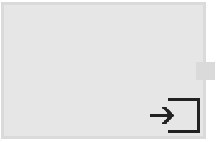
\includegraphics[height=60px]{figures/SourceOperator.pdf}
	\caption{Source operator representation.}
	\label{fig:source operator}
\end{figure}

Source operators together with processing operators are the ones that can be 
used to specify data flow coming out of an operator. Output specification is an 
action to identify the data tuple with a series of segments. Other operator types 
cannot make changes on output specification, but can manipulate the flow by dropping 
or copying data tuples.

\textbf{human.} 
The \textit{human source operator} is a stateless operator used to produce new data tuples 
via human workers. Existing crowdsourcing services such as MTurk is used 
to produce new tuples. A new data tuple is produced per successfully completed 
human intelligent task. These tasks are automatically created and posted with 
respect to the specified parameters of the operator.

Human source operator has the following parameters:
\begin{itemize}
	\item \texttt{number of copies}: The maximum number of data tuples can be 
	generated by the operator. It's value ranges from 1 to 1000.
	\item \texttt{max allotted time}: The maximum time in seconds given to a human 
	worker to solve and submit the task. It's value ranges from 10 to 300.
	\item \texttt{lifetime}: The life time of human task in hours during which period 
	task will be available to human workers. It's value ranges from 1 to 72.
	\item \texttt{payment}: The payment in cents to be given to the human worker in 
	case of successful task completion. It's value ranges from 5 to 500.
	\item \texttt{instructions}: The detailed information for human workers on how to 
	complete the task.
	\item \texttt{question}: The set of sentences asking for specific information from 
	human workers.
	\item \texttt{input list}: The list of \texttt{input}s that will be shown to human worker 
	to fill in. An \texttt{input} can be a type of \textit{text, number, single choice} or 
	\textit{multiple choice}. Each of these types corresponds to an HTML element. 
	Table~\ref{tab:input list} lists types and their details.
	
	A text-input presents an input field where the human worker can 
	enter data. The maximum number of characters that can be entered to the field can be 
	set by the requester. Similarly number-input corresponds to a input field where only 
	numbers can be fed in, and the maximum and minimum value for the field are set by 
	the requester. The other two input types conform to input fields where the options given 
	by the requester are presented to the human worker as a list. Human worker is expected 
	to select only one and one or more options for single choice and multiple choice types 
	respectively.
	
	In fact, each \texttt{input} conforms to a segment in the data tuple.
\end{itemize}

\begin{table}[ht]
	\centering
	\caption{List of inputs and options}
	\label{tab:input list}
	\begin{tabular}{| l | l | l |}
		\hline
		type & parameters & HTML element \\ \hline
		text & max number of characters & input [type=text] \\ \hline
		number & min value, max value & input [text=number] \\ \hline
		single choice & options & input [type=radio] \\ \hline
		multiple choice & options & input [type=checkbox] \\ \hline
	\end{tabular}
\end{table} 


%This operator has a significant role in the platform. 
% platform-independence, abstracts away the details of the underlying platform
% use results of other operators
% customize collaboration by specifying audience

\textbf{manual.}
The \textit{manual source operator} is a stateless operator to produce new data 
tuples.

\newcommand{\ditto}{\texttt{\char`\'}}

Manual source operator has the following parameters:
\begin{itemize}
	\item \texttt{manual entry}: The manual text to be parsed and used to produce 
	new tuples.
	\item \texttt{delimiter}: Delimiter to determine segments in a tuple. This can have one 
	of the following values: none (\ditto\ditto), white space (\ditto\texttt{ }\ditto), 
	tab (\ditto\texttt{\char`\\t}\ditto), comma (\ditto\texttt{,}\ditto), 
	column (\ditto\texttt{:}\ditto).
\end{itemize}

Manual source operator uses manually entered text to create new tuples. Operator 
retrieves the manual text, parses it line by line and then applies the delimiter. 
Therefore, each line constitutes a data tuple, and delimiter is used to create segments 
in a tuple.

For example, if \texttt{delimiter} is chosen to be white space and the following is 
entered to \texttt{manual entry},

\begin{lstlisting}
Lorem ipsum
Consectetur adipiscing
Phasellus vehicula
\end{lstlisting}

\noindent the following data tuples will be generated:

\begin{lstlisting}
[
{"segment_1": "Lorem", "segment_2": "ipsum"},
{"segment_1": "Consectetur", "segment_2": "adipiscing"},
{"segment_1": "Phasellus", "segment_2": "vehicula"}
]
\end{lstlisting}

It is possible to have such a manual entry that ends up in different number of segments 
for different lines. To prevent this happening manual source operator uses the first line 
to generate output specification. If more segments are generated in the following lines, 
they are discarded. If there are not enough segments in another line, then the corresponding 
segments are emptied and then outputted.

\subsection{Sink operators}
The set of sink operators is where data tuples are serialized and converted into 
the formats that can be used by requesters with ease. These operators have one 
input port, but no output port. Figure \ref{fig:sink operator} demonstrates a sink operator.

\begin{figure}[ht]
	\centering
	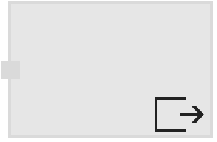
\includegraphics[height=60px]{figures/SinkOperator.pdf}
	\caption{Sink operator representation.}
	\label{fig:sink operator}
\end{figure}

\textbf{email.}
The \textit{email sink operator} is a stateless operator to convert data tuples into a 
text format and email them to requesters. \texttt{email} parameter specifies the 
requester's email address. 

\textbf{file.}
The \textit{file sink operator} is a stateless operator to serialize the data tuples into 
a file. Operator has one parameter \texttt{filename} that is used to specify the name 
of file in which tuples will be written.

\subsection{Processing operators}
The set of processing operators provides data tuple processing via human workers. 
These operators have both input and output ports. Figure \ref{fig:processing operator} 
shows a processing operator.

\begin{figure}[ht]
	\centering
	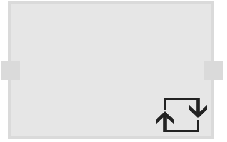
\includegraphics[height=60px]{figures/ProcessingOperator.pdf}
	\caption{Processing operator representation.}
	\label{fig:processing operator}
\end{figure}

As mentioned before, processing operators can manipulate the data flow specification 
in addition to source operators. These operators can change the existing flow specification 
by adding, deleting or editing data segments.

\textbf{human.}
The \texttt{human processing operator} is almost same as human source operator. 
The difference is human processing operator has an input port. That means there is a 
flow of data tuples coming to operator. These incoming tuples are made available 
to requesters via their specification.

The parameters of human processing operator is no different than the parameters of 
human source operator. Additionally processing operator has available segment list, which 
provides placeholders for the segments of an incoming data tuple. Requesters can place 
these placeholders in \texttt{instructions}, \texttt{question} and \texttt{input list} 
(applicable to single choice and multiple choice inputs).

At runtime when a new tuple arrives, each placeholder in parameters is replaced with 
the corresponding value of incoming tuple's segment. This enables dynamically created human 
tasks. Therefore, requesters can create an information flow from one operator to another.

\subsubsection{Relational operators}
The set of relational operators enables fundamental manipulation operations on 
the flow of data tuples. Each relational operator implements a specific functionality 
providing continuous and non-blocking processing on tuples. Therefore, these operators 
have both input and output port.

\textbf{selection.}
The \textit{selection operator} is a stateless operator used to filter tuples. A typical 
selection operator is shown in Figure~\ref{fig:selection operator}.

\begin{figure}[ht]
	\centering
	
\includegraphics[height=60px]{figures/SelectionOperator.pdf}
	\caption{Selection operator representation.}
	\label{fig:selection operator}
\end{figure}

On a per-tuple basis a boolean predicate is evaluated and a decision is made as 
to whether to filter the corresponding tuple or not. Boolean predicates are specified 
by requesters as part of operator parameterization. These predicates, which are 
identified in \texttt{rules}, are the only members of parameters.

A selection operator has zero or more rules to filter data tuples. When there is 
no rule specified, then no filtering will be done, and all data tuple will be passed 
down to data flow. Otherwise, each rule is evaluated on an incoming data tuple. 
Whenever a rule is evaluated to be true, then corresponding action is carried out 
that is either filter in or out the tuple, and the rest of rules is discarded. If no rule is 
evaluated to be true on a data tuple, then tuple is still passed to the next operator(s). 
Rules share the following predefined format:

\textit{Filter} \textit{(in/out)} \textit{when} \texttt{boolean-predicate}

Similarly \texttt{boolean-predicate} has the following format

\texttt{segment-name} \textit{(equals/not equals/contains)} \texttt{query}

where \texttt{segment-name} is one of the segments of incoming tuple, 
and \texttt{query} is a free-text to be filled by requester.

\textbf{sort.}
The \textit{sort operator} is a stateful and windowed operator used to first group 
tuples and then sort them based on the specified data segment and order. Figure
~\ref{fig:sort operator} illustrates the operator.

\begin{figure}[ht]
	\centering
	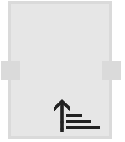
\includegraphics[height=60px]{figures/SortOperator.pdf}
	\caption{Sort operator representation.}
	\label{fig:sort operator}
\end{figure}

Sorting is performed and results are produced (outputted one by one) every time 
window trigger policy fires. The policy is basically triggered when the number of 
data tuples reaches \texttt{window size}, which is specified as a parameter. 
\texttt{window size} can have a value between 1 and 100.

Similar to selection operator, sort operator implements a set of rules that simply 
identifies the segment and the order to be used for sorting. If no rule is specified, 
then tuples are sorted in the ascending order with respect to the first segment in 
the incoming data tuples. If there are more than one rule is given, then these rules 
are applied in the order they are specified by requester.

Sorting rules share the following predefined format:

\textit{Sort using} \texttt{segment-name} \textit{in} \textit{(ascending/descending)} \textit{order}

where \texttt{segment-name} is one of the segments of incoming tuple.

\subsection{Utility operators}
\label{sec:utility operators}
The set of utility operators provides flow management functions. These operators 
handle operations such as separating a flow into multiple flows or joining multiple 
flows into a single one.

\textbf{enrich.}
The \textit{enrich operator} is a stateless operator used to enrich data flow by 
replaying incoming data tuples. Figure~\ref{fig:enrich operator} shows an example 
view of the operator.

\begin{figure}[ht]
	\centering
	
\includegraphics[height=60px]{figures/EnrichOperator.pdf}
	\caption{Enrich operator representation.}
	\label{fig:enrich operator}
\end{figure}

Enrich operator has one parameter called \texttt{number of copies}. This parameter 
determines how many copies will be produced for each incoming tuple. It's value 
ranges from 1 to 10.

\textbf{split.}
The \textit{split operator} is a stateless operator used to divide an inbound flow 
into multiple flows. This operator has one incoming flow and and can have one or 
more outgoing flow. Figure~\ref{fig:split operator} provides the presentation of a 
split operator.

\begin{figure}[ht]
	\centering
	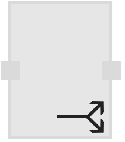
\includegraphics[height=60px]{figures/SplitOperator.pdf}
	\caption{Split operator representation.}
	\label{fig:split operator}
\end{figure}

The boolean predicates specified in rules are evaluated whenever a new tuple 
arrives. Then, a decision is made to where to send the tuple. Similar to relational 
operators, rules are specified by requesters as part of operator 
parameterization.

A split operator has zero or more rules. When there is no rule specified, then 
tuples are passed to every operator connected down the flow. Otherwise, each 
and every rule is evaluated on an incoming data tuple. Whenever rule's predicate 
is evaluated to be true, then tuple is passed to the corresponding operator. If no 
predicate turns out to be true for a tuple, then it is dropped.

It is possible that more than one rule for the same \texttt{next-operator} can be true 
for a specific data tuple. This doesn't mean that tuple will be sent to that operator 
multiple times. Only one tuple will be outputted to \texttt{next-operator}.

Rules share the following predefined format:

\textit{Send to} \texttt{next-operator} \textit{when} \texttt{boolean-predicate}

in which \texttt{next-operator} is the connected operators down the flow, and 
\texttt{boolean-predicate} has the same definition given for selection operator.

\textbf{union.}
The \textit{union operator} is a stateless operator used to join two or more data flows 
into one. Different than other operators, this operator can receive more than one flow. 
These flows are combined by the operator and outputted as if they are a single flow. 
Figure~\ref{fig:union operator} demonstrates the operator.

\begin{figure}[ht]
	\centering
	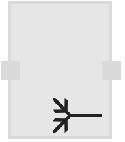
\includegraphics[height=60px]{figures/UnionOperator.pdf}
	\caption{Union operator representation.}
	\label{fig:union operator}
\end{figure}

Union operator requires incoming flows to have the same specification. Otherwise, 
union operation will basically fail.

\section{Flow}
Flow is the connection between operators used to move information from one operator 
to another. A flow is formed by one or more data segments. A segment has an identifier 
and corresponding value. In that sense, flow is like a hash table where segment identifiers 
are keys, and values stored in segments are values as demonstrated in the following:

\begin{lstlisting}
{
"segment-1": "value-1",
"segment-2": "value-2",
...
"segment-N": "value-N",
}
\end{lstlisting}

The details of a flow can be specified by either source or processing operators. It is 
immutable in other operators. Specification can be achieved via output specification section 
in operator configuration. Requesters can create new segments, edit or delete existing ones. 
Source operators are useful to specify flow specification in the early stages of workflow 
design and generate tuples using that specification. The flow specification is crucial, since 
it determines the specifics of the information that is carried over in the application. Still this 
specification can be redefined in processing operators.

\section{Application Development}
\label{sec:flow comp}
The application development using $Crowdy$ can be achieved by simply creating new 
operators, configuring them and connecting them together. However, there are certain 
predefined rules that should be satisfied to develop a valid application and execute it.

An application is formed by a workflow. Although it is not suggested, application can have 
multiple workflows. A workflow is basically a set of operators connected together. An operator 
can be connected to another operator by attaching a flow from the output port of an operator 
to the input port of the other operator. Workflow must contain at least one source and one 
sink operator. There may be operators that are not connected to any 
other operator within the application. Operators with no connections are discarded and 
they do not cause validation failures.


A valid workflow means that each each operator employed in that workflow is valid. Validity of 
an operator depends on it's type and therefore it's configuration. In the following each operator 
group is examined in terms of validation.

\subsubsection{Source operators}
A source operator has one output port, which outputs the data tuples with given specification. 
Therefore, source operator is required to have an output specification that has at least one data 
segment in it.

\textbf{human.} 
Parameters of a human operator should be valid. That means 
\texttt{number of copies} is an integer between 1 and 1000, 
\texttt{max allotted time} is an integer between 10 and 300, 
\texttt{payment} is an integer between 5 and 500. 
Although \texttt{instructions} can be left empty by the requester, \texttt{question} cannot be 
empty. There must be at least one \texttt{input} defined in the \texttt{input list} to satisfy that 
source operators have an output specification with at least one segment defined.

\textbf{manual.} 
\texttt{manual entry} and \texttt{delimiter} should not be empty. Nonempty \texttt{manual entry} 
and \texttt{delimiter} correspond to an output specification with at least one segment in it.

\subsubsection{Sink operators}
A sink operator has one input port, which receives data tuples.

\textbf{email.} 
Operator must have a valid email address given in \texttt{email} parameter.

\textbf{file.} 
Operator must have a valid file name given in \texttt{filename} parameter.

\subsubsection{Processing operators}
A processing operator has one input and one output port. It receives data tuples, processes 
them and outputs them to next operator down to flow. Similar to source operators, processing 
operators must have an output specification that has at least one data segment in it. Since 
human operator is the only processing operator, the validity rules for this operator is same as 
human operator of type source operator.

\subsubsection{Relational operators}
A relational operator has one input and one output port. It is useful to manipulate flow. 
Operators of this type has rules to determine manipulation.

\textbf{selection.}
Each rule in the rule list must be valid, which means a rule with valid \texttt{segment-name}.

\textbf{sort.}
Operator must have a valid \texttt{window size}. This value can be an integer between 
1 and 100. Additionally each rule in the rule list must be valid by being formed by a valid 
\texttt{segment-name}.

\subsubsection{Utility operators}
A relational operator has one input and one output port. This type of operators is useful for 
flow management.

\textbf{enrich.}
Operator must have a valid \texttt{number of copies}. This value can be an integer between 
1 and 10.

\textbf{split.}
Split operator must have an incoming flow to-be-splitted and at least one outgoing flow. 
Split operation is defined by rules. Each rule in the rule list must be valid by specifying 
a valid \texttt{next-operator}.

\textbf{union.}
Union operator must have at least one incoming flow to-be-merged and one outgoing flow. 
Each incoming flow must have the same specification, which is ensured by application editor 
by preventing connecting flows with different specification to the same union operator.



\chapter{Tool}
\label{sec:tool}
$Crowdy$ has been implemented as a web-based tool and made freely 
available\footnote{http://crowdy.herokuapp.com}. The 
client part of the tool is developed using Javascript, while application server and 
virtual machine is written in python. The tool is deployed to Heroku 
\footnote{http://www.herokuapp.com} cloud application 
platform. The tool can be used by anyone to solve a problem that requires both 
software and human resources. In terms of crowdsourcing parlance users of the tool 
is called \textit{requesters}.

Requesters can use $Crowdy$ to define and configure crowdsourcing applications. 
In this section, the application development over $Crowdy$ platform is 
demonstrated using the tool. The minimal example application presented earlier 
in this section is implemented. The steps are presented and explained in detail 
with the sample screenshots from the tool.

A $Crowdy$ application consists of operators in which one is connected to the other creating 
an information flow. Figure~\ref{fig:panel1} shows the flow composition panel of the tool, which 
is used to create and configure applications. At the top (pointed by (1)), a simple set of 
instructions is listed to help users in the application development process. Additionally links 
to validate an application, clear the flow composition panel and report a bug are given here. 
On the left (pointed by (2)), the list of operators is given and that list is separated by operator 
type, which is described in detail earlier in this section. The panel (pointed by (3)) is where 
operators are placed and linked together to develop an application. Finally, the messages 
panel (pointed by (4)) is where important information about the application are displayed to 
user such as warnings, validation failures or successes etc.

\begin{figure}[ht]
	\centering
	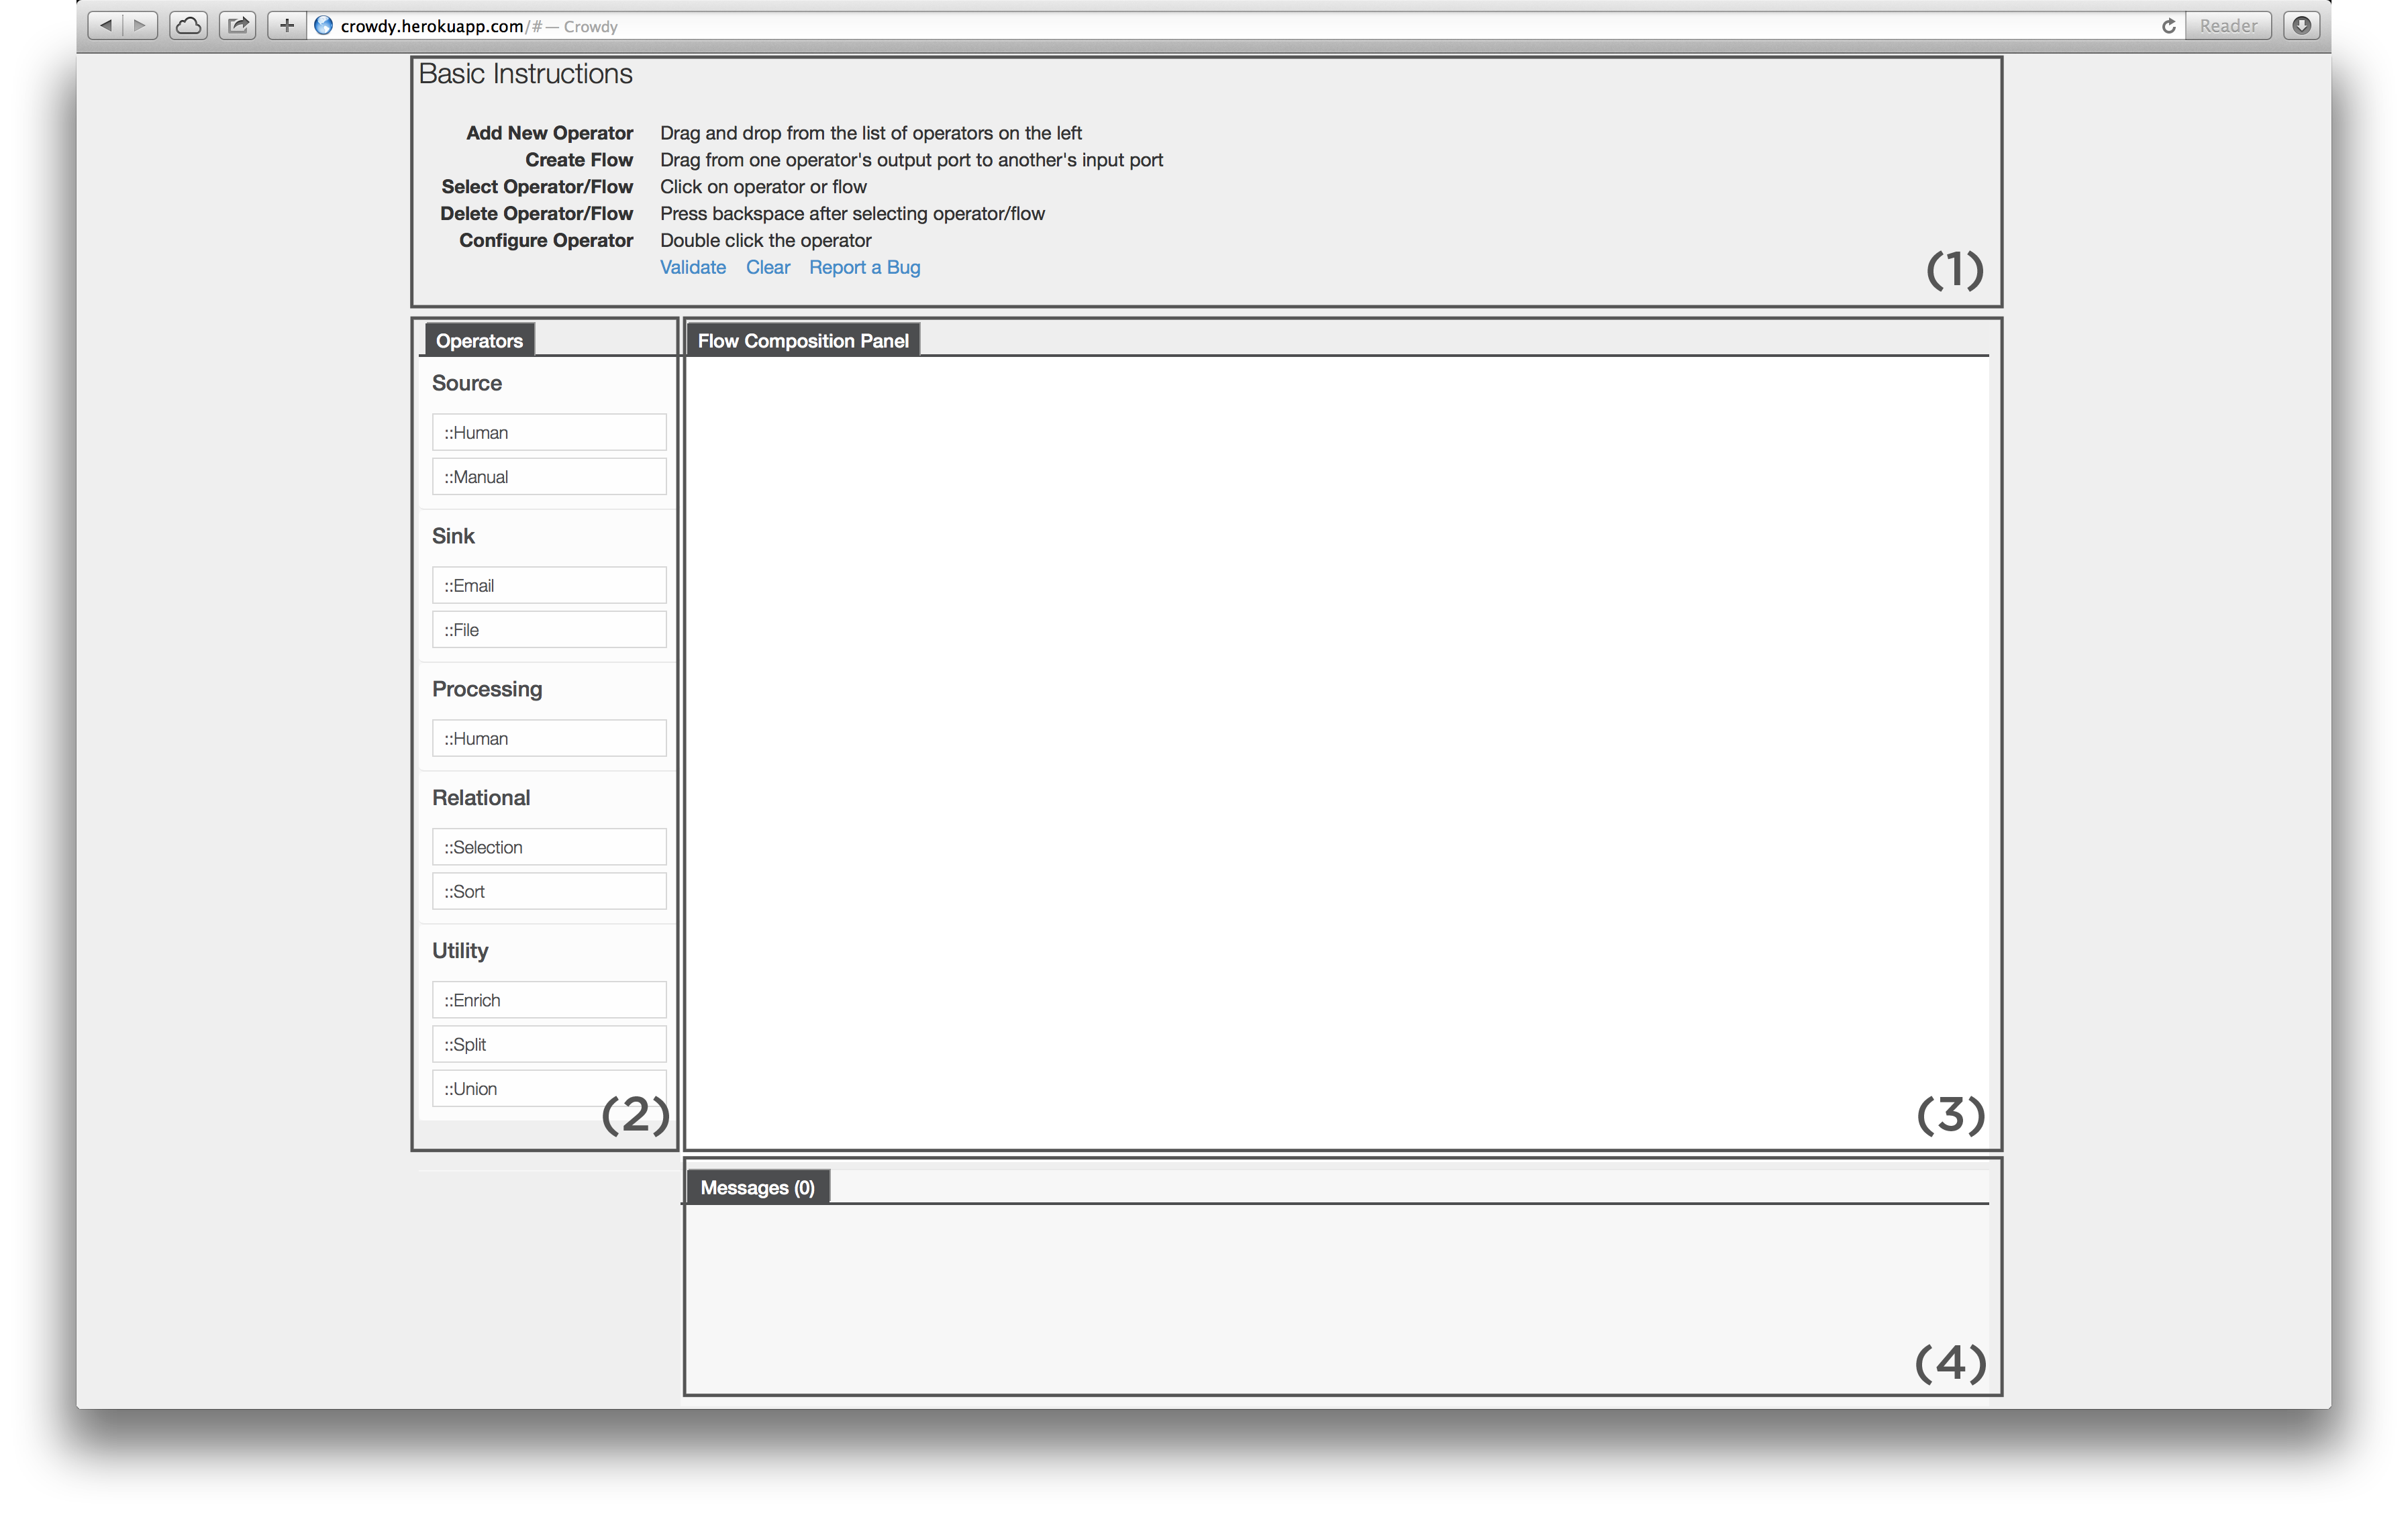
\includegraphics[width=0.9\textwidth]{figures/tool/panel1.png}
	\caption{Flow composition window.}
	\label{fig:panel1}
\end{figure}

The creation of an operator is simple in $Crowdy$. Operators are created by dragging and 
dropping the specific operator from the list to the panel. An operator can be moved across 
the panel freely by dragging. An operator can be selected and deselected by clicking the 
operator body. Once an operator is selected, the border color of the operator is darkened 
to indicate it is actually selected. A selected operator can be removed by 
pressing backspace key in the keyboard. Figure~\ref{fig:panel2} shows that a source 
operator is created and selected.

\begin{figure}[ht]
	\centering
	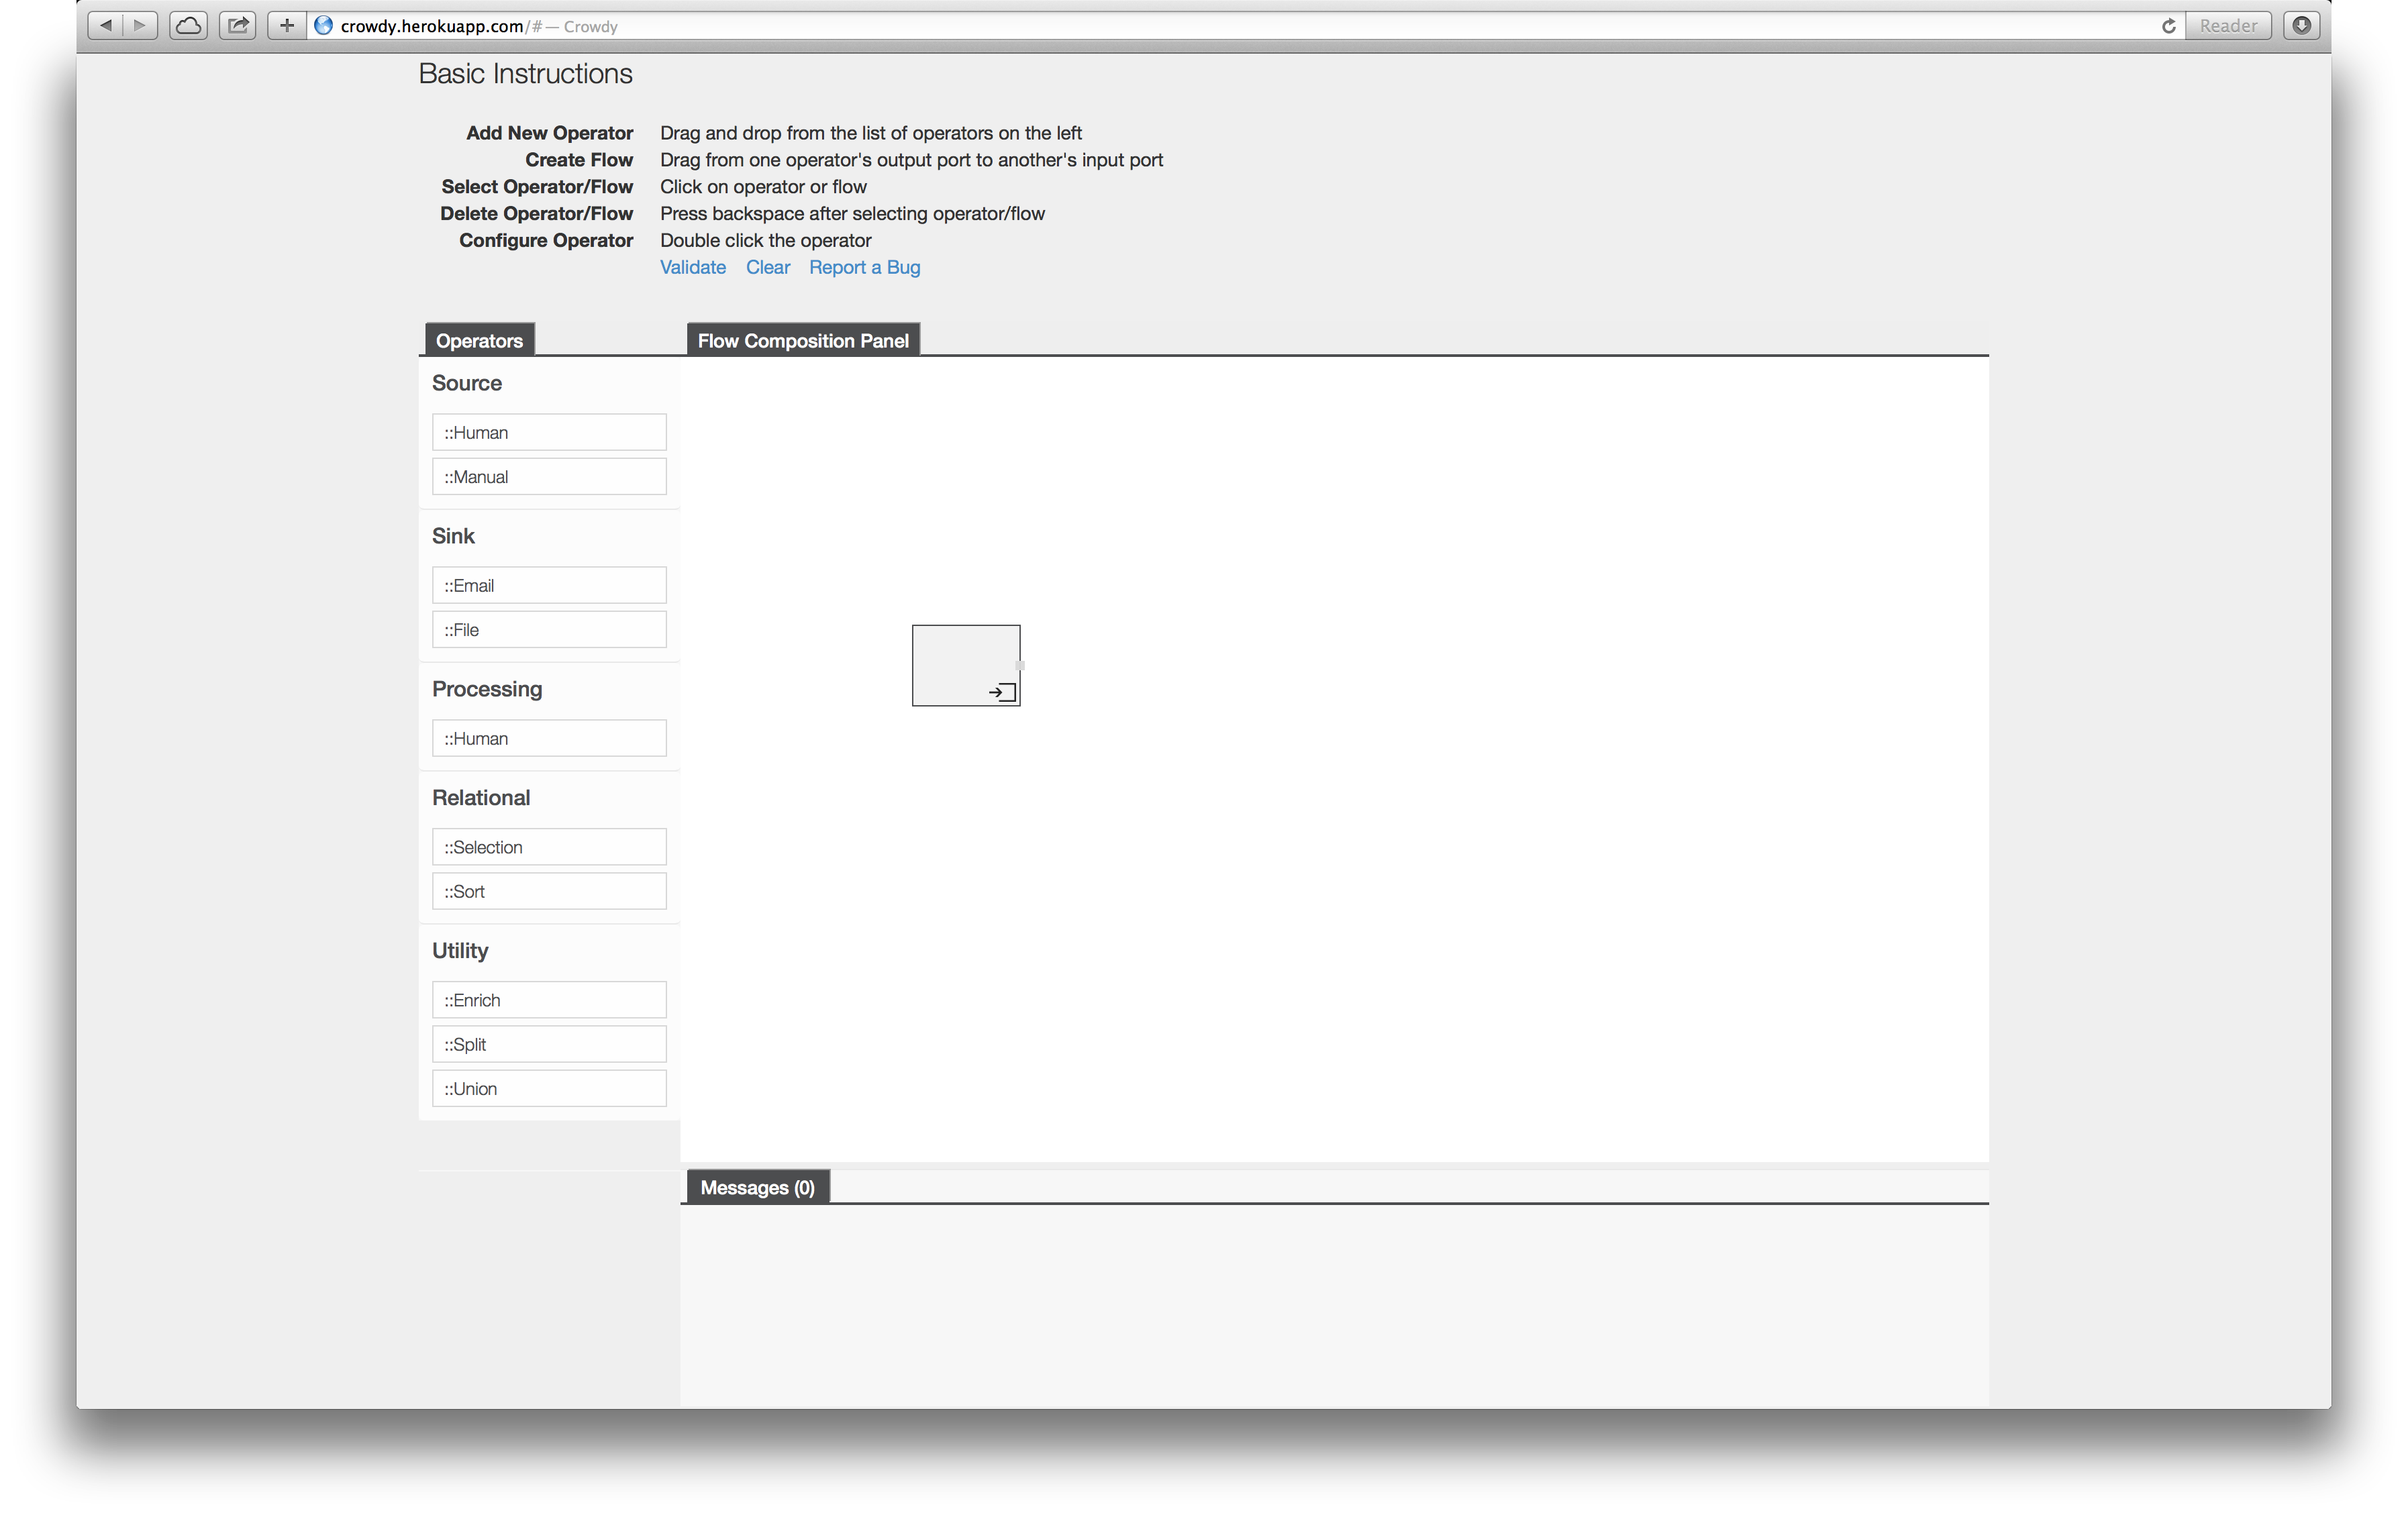
\includegraphics[width=0.9\textwidth]{figures/tool/panel2.png}
	\caption{An source operator added to flow.}
	\label{fig:panel2}
\end{figure}

As explained in Section~\ref{sec:operator} in a detailed manner, operators in $Crowdy$ 
are easily configurable. Each operator has it's own definition of configuration and list 
of options. This configuration window can be opened by double-clicking operator body. 
Figure~\ref{fig:panel3} demonstrates the configuration window for
\textit{source manual operator}. The configuration has three sections: \textit{details}, 
\textit{parameters} and \textit{output specification}. The \textit{details} section exists for 
every operator and it can be used for bookkeeping purposes such as assigning 
names, noting some information specific to those operators. The \textit{parameters} 
section is specific to each operator and this is where actual configuration per operator 
can be achieved. In this example, configuration for \textit{source manual operator} 
is depicted. Finally, the \textit{output specification} section is where output definition 
of that operator is shown. This section lists the data segments for that operator. These 
segments can be renamed by clicking and editing the names. This section is 
not shown for \textit{sink operators}, since they don't have any output to be delivered 
to some other operator. In fact, this section is automatically generated for 
\textit{relational} and \textit{utility operators} and updated once the source of those 
segments makes any changes, since they are able capable of changing the 
output specification by adding or deleting new segments.

\begin{figure}[ht]
	\centering
	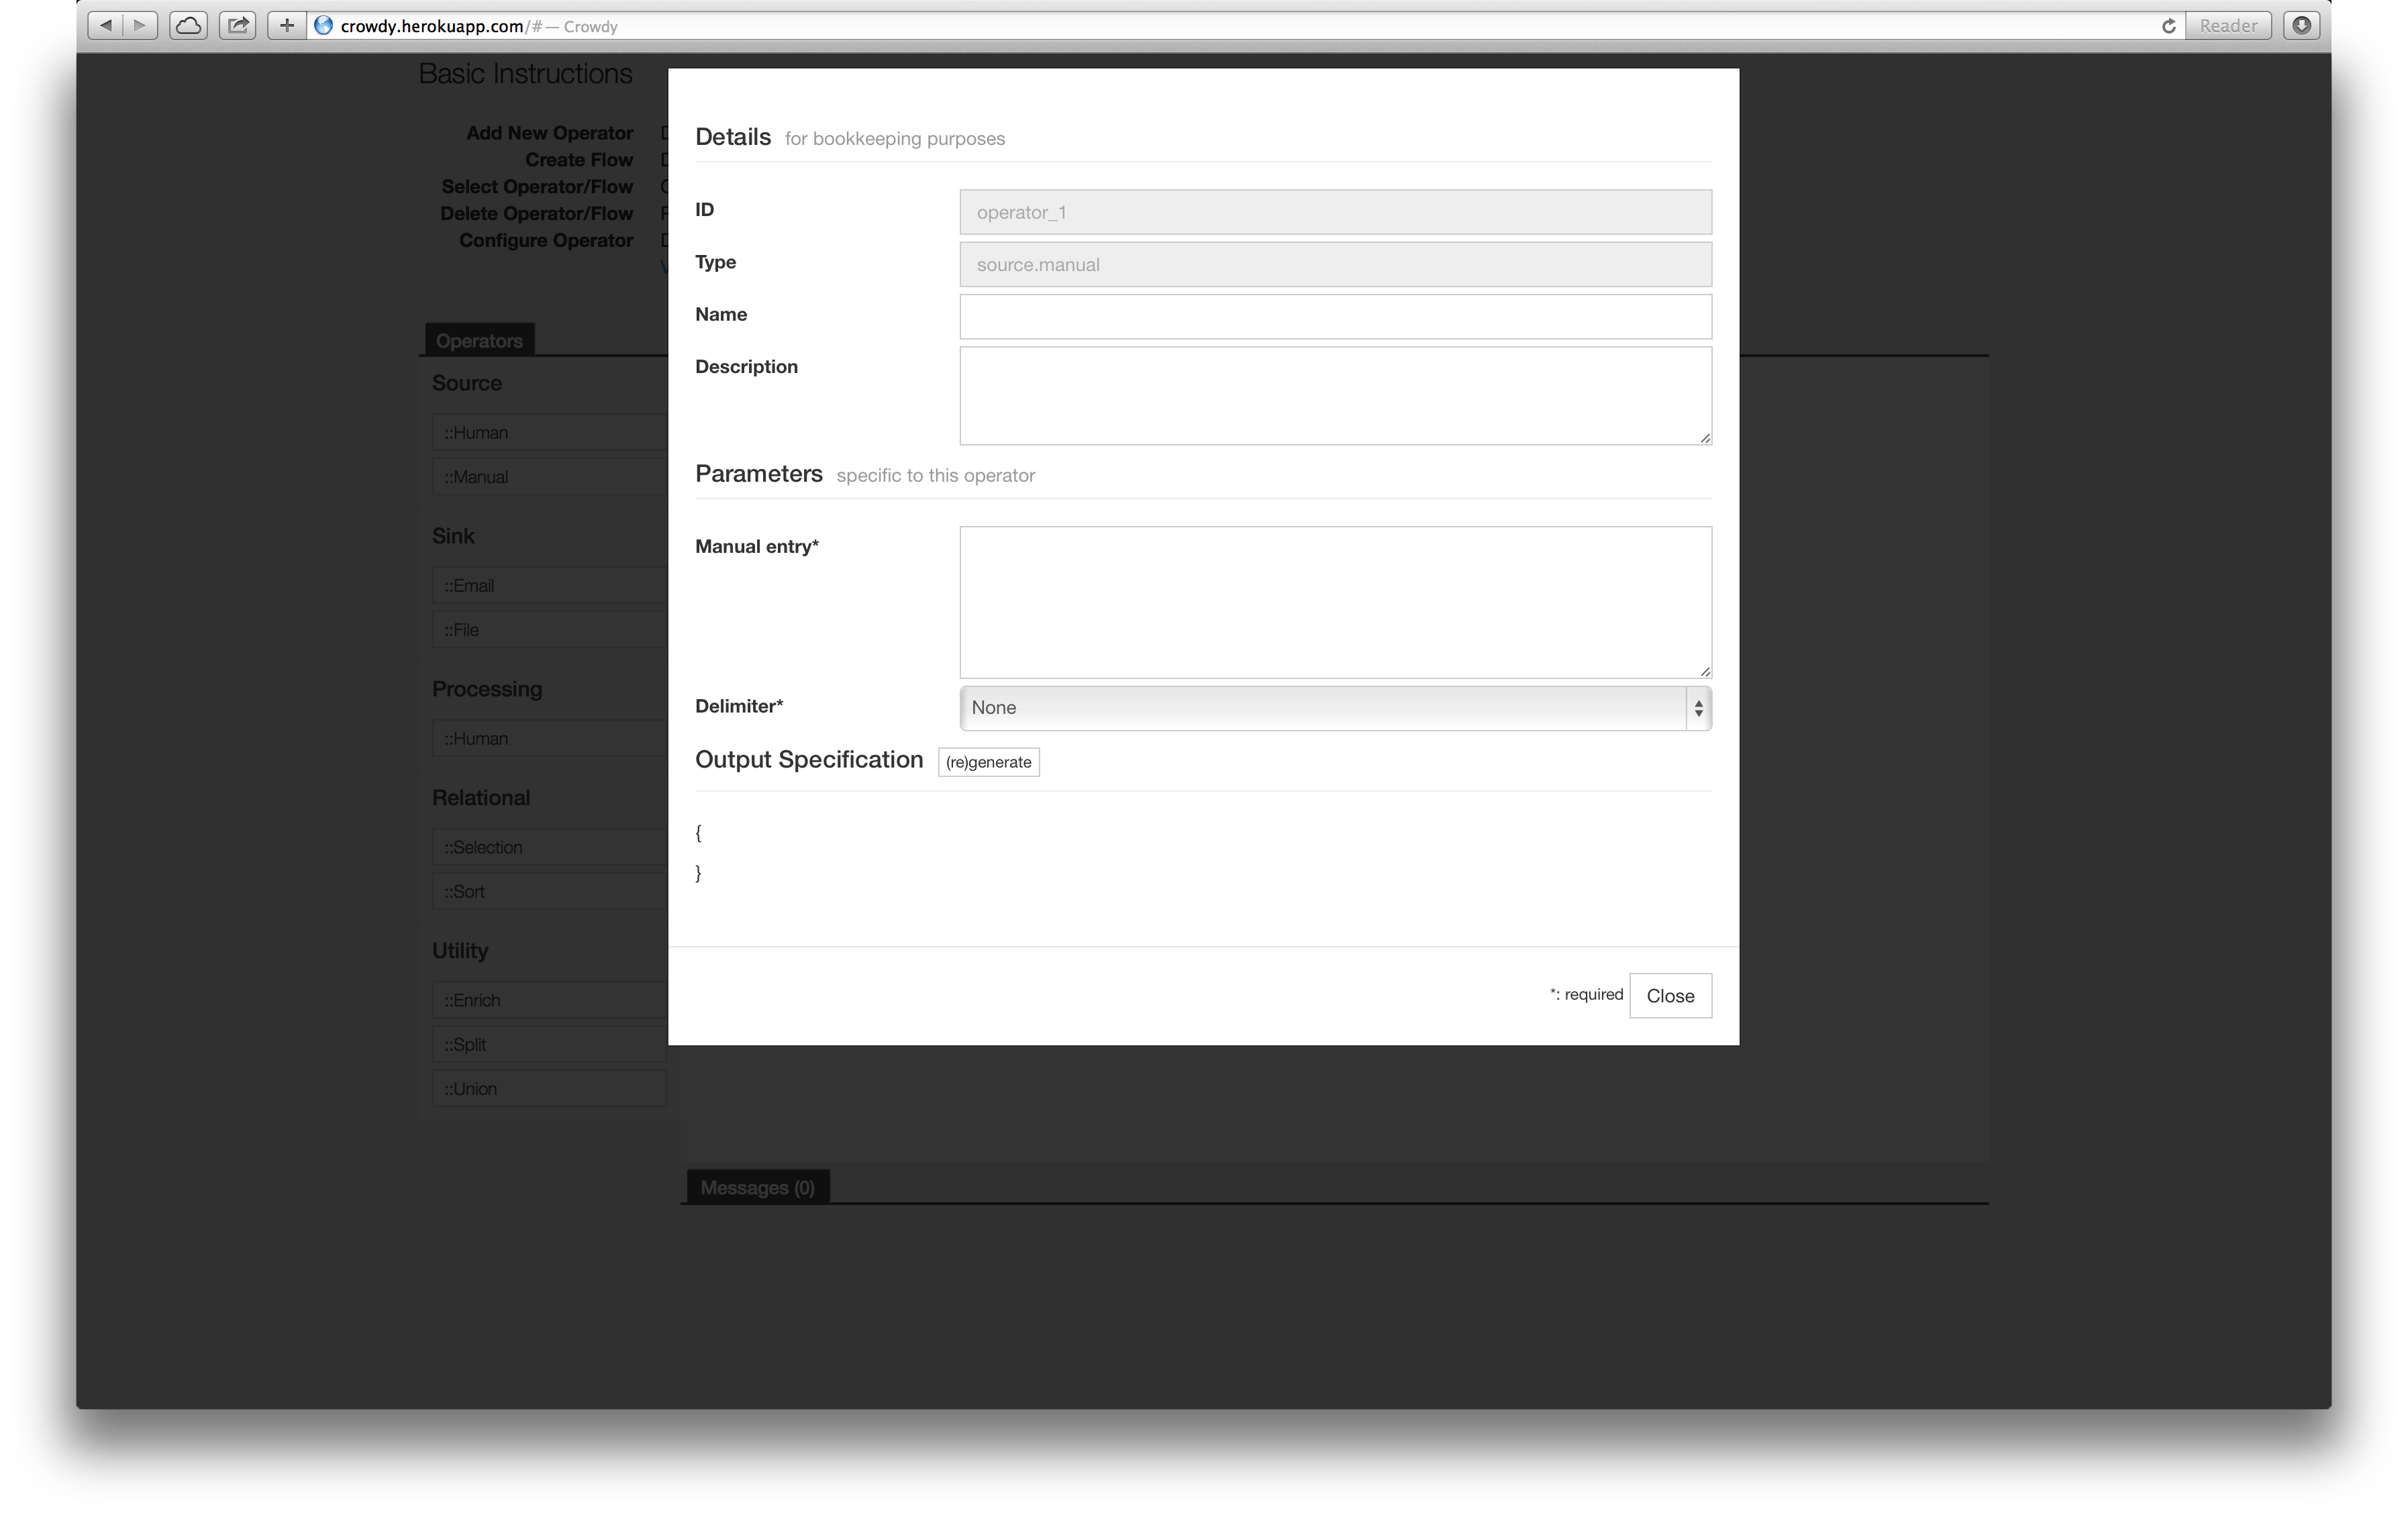
\includegraphics[width=0.9\textwidth]{figures/tool/panel3.png}
	\caption{Configuration window for source manual operator.}
	\label{fig:panel3}
\end{figure}

Figure~\ref{fig:panel4} redemonstrates the configuration window, but 
now fields are complete and outputs are specified. To exemplify the functionality 
the list of countries and capitals separated by tab is entered. Delimiter is selected 
to be tab in that sense and output specification is automatically generated. The 
data segments are renamed after the information they are containing. The 
segment names will be useful down the flow while creating human tasks or 
manipulating flow of information.

\begin{figure}[ht]
	\centering
	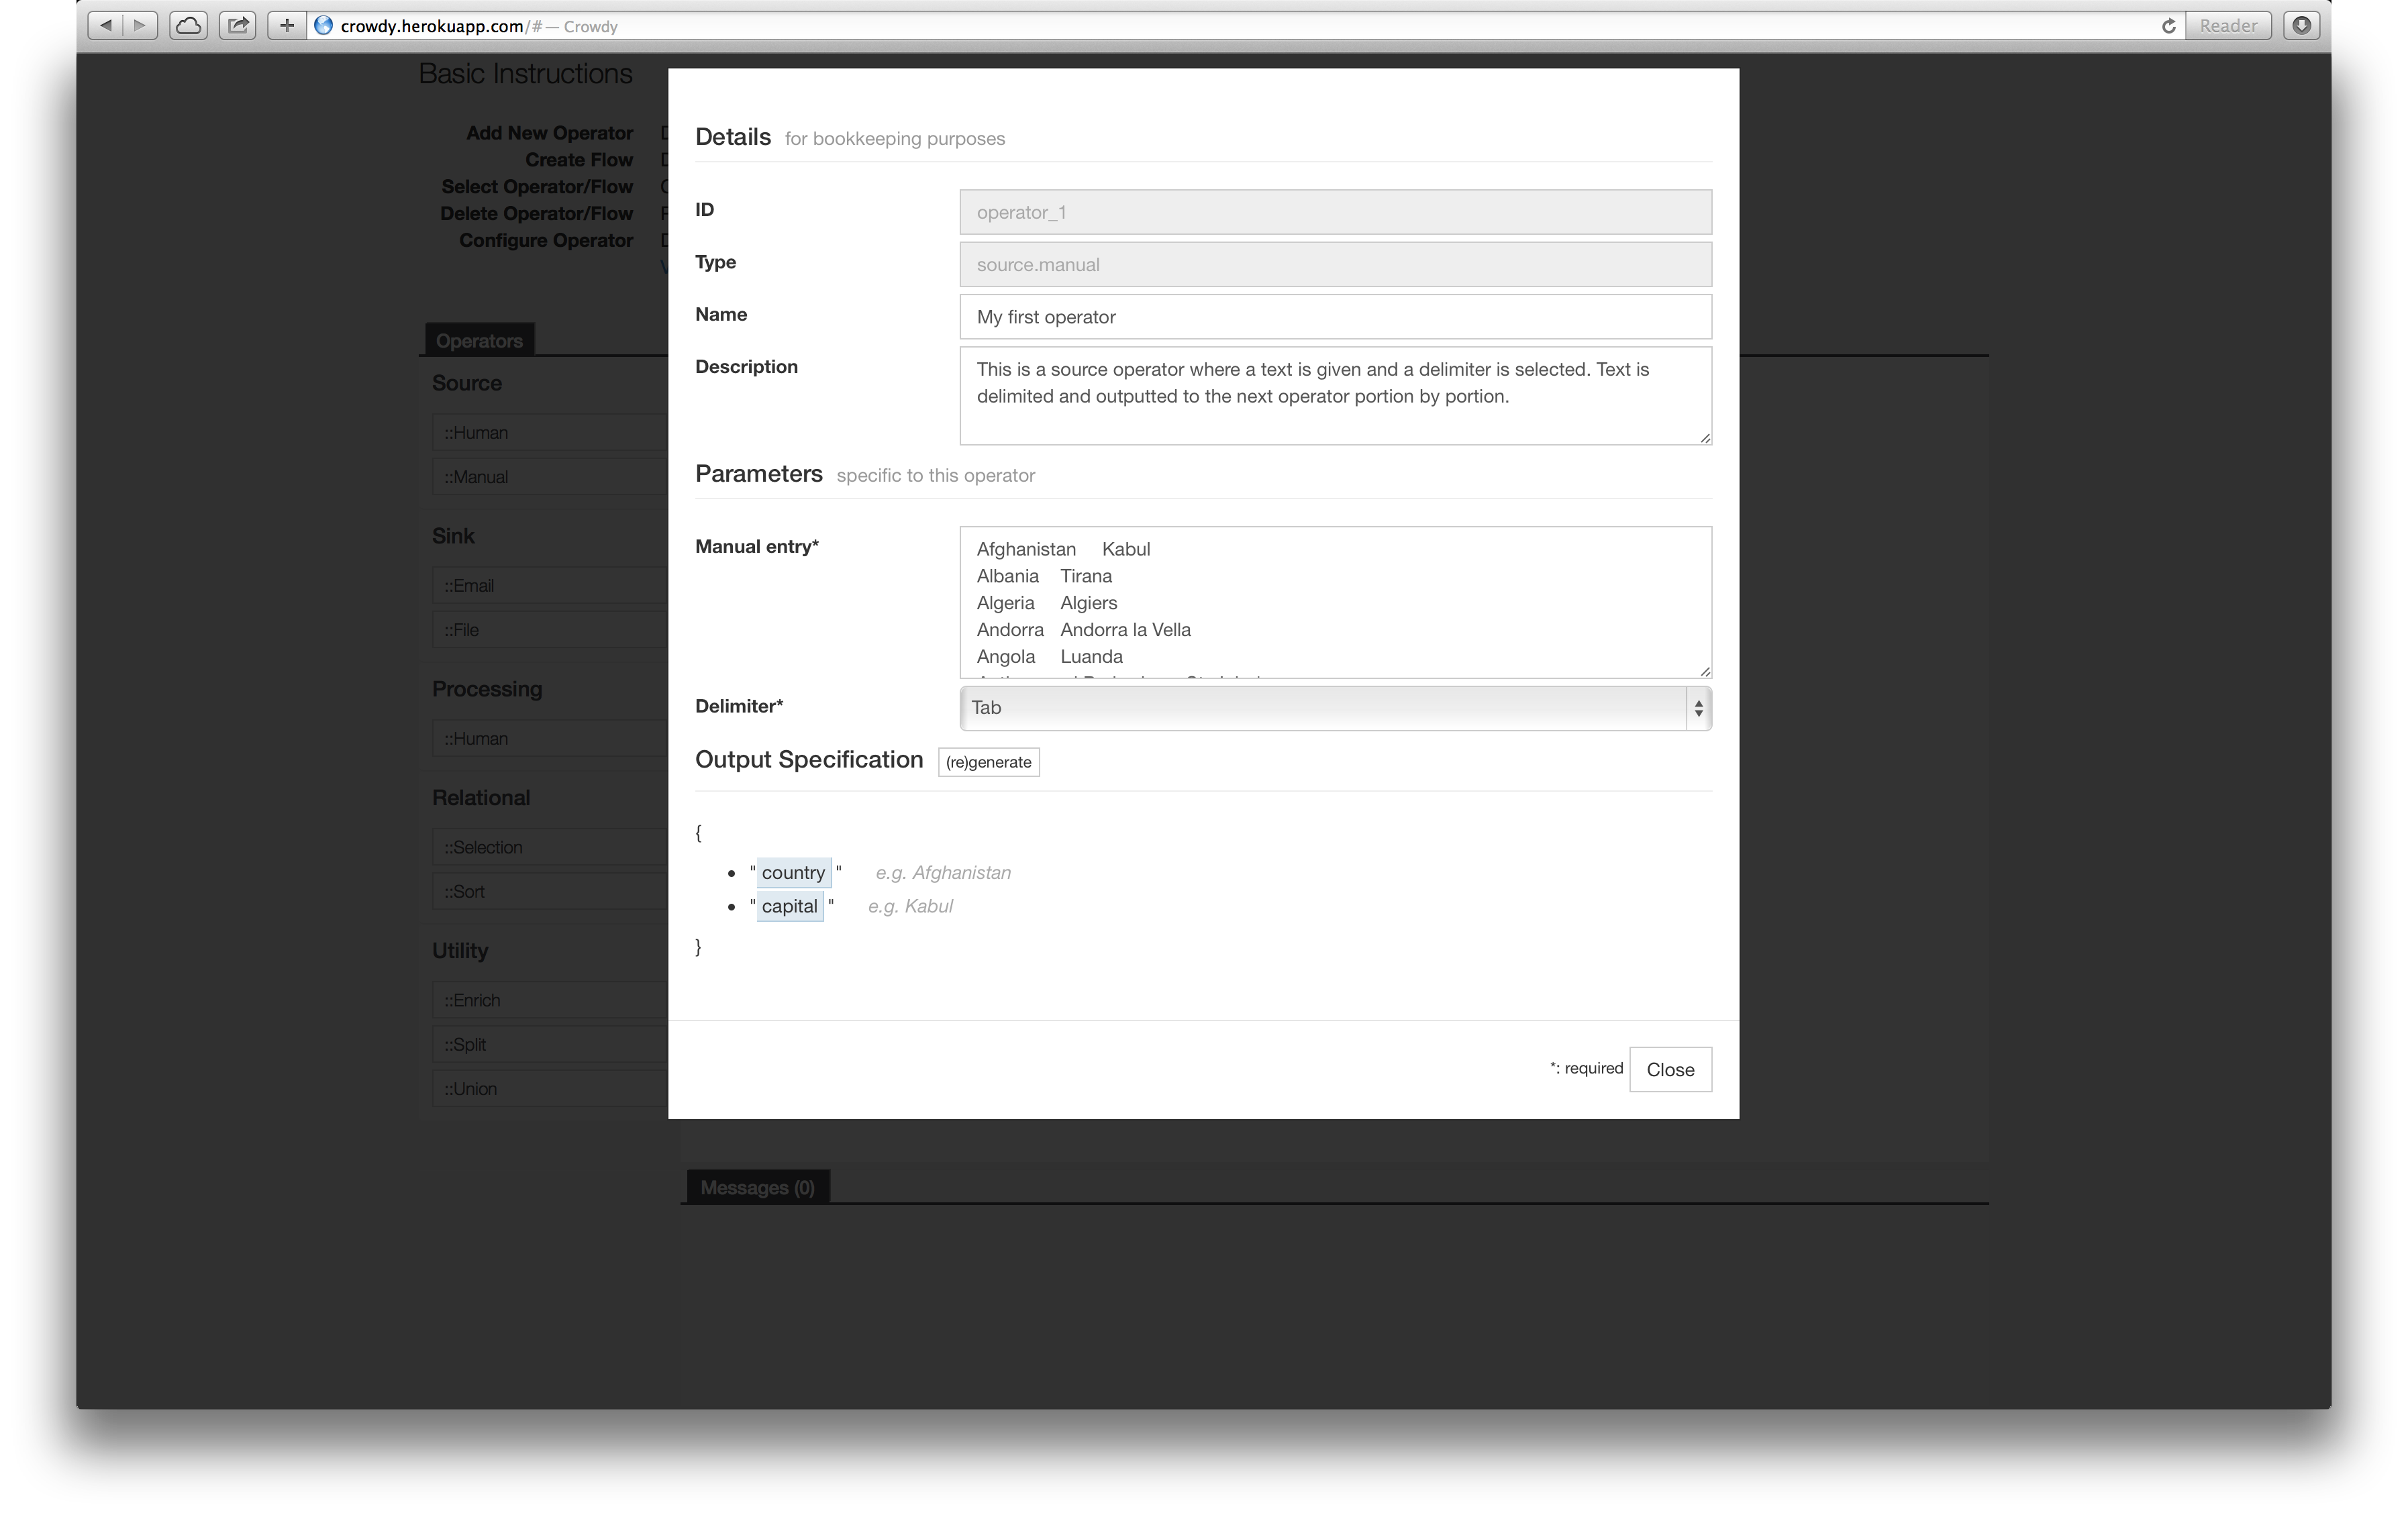
\includegraphics[width=0.9\textwidth]{figures/tool/panel4.png}
	\caption{Configuration window for source manual operator filled with sample information.}
	\label{fig:panel4}
\end{figure}

The \textit{human processing operator} is created and then the output of source 
operator is connected to it to create the flow as shown in Figure~\ref{fig:panel5}. 
The arrow on the flow shows the direction of information. Similar operator 
selection and deletion operations, the flow (the link between operators) can 
be selected and deselected by clicking. A selected flow can be removed by 
pressing backspace key in the keyboard. Once a flow is deleted, the connected 
operators to that flow are deleted as well.

\begin{figure}[ht]
	\centering
	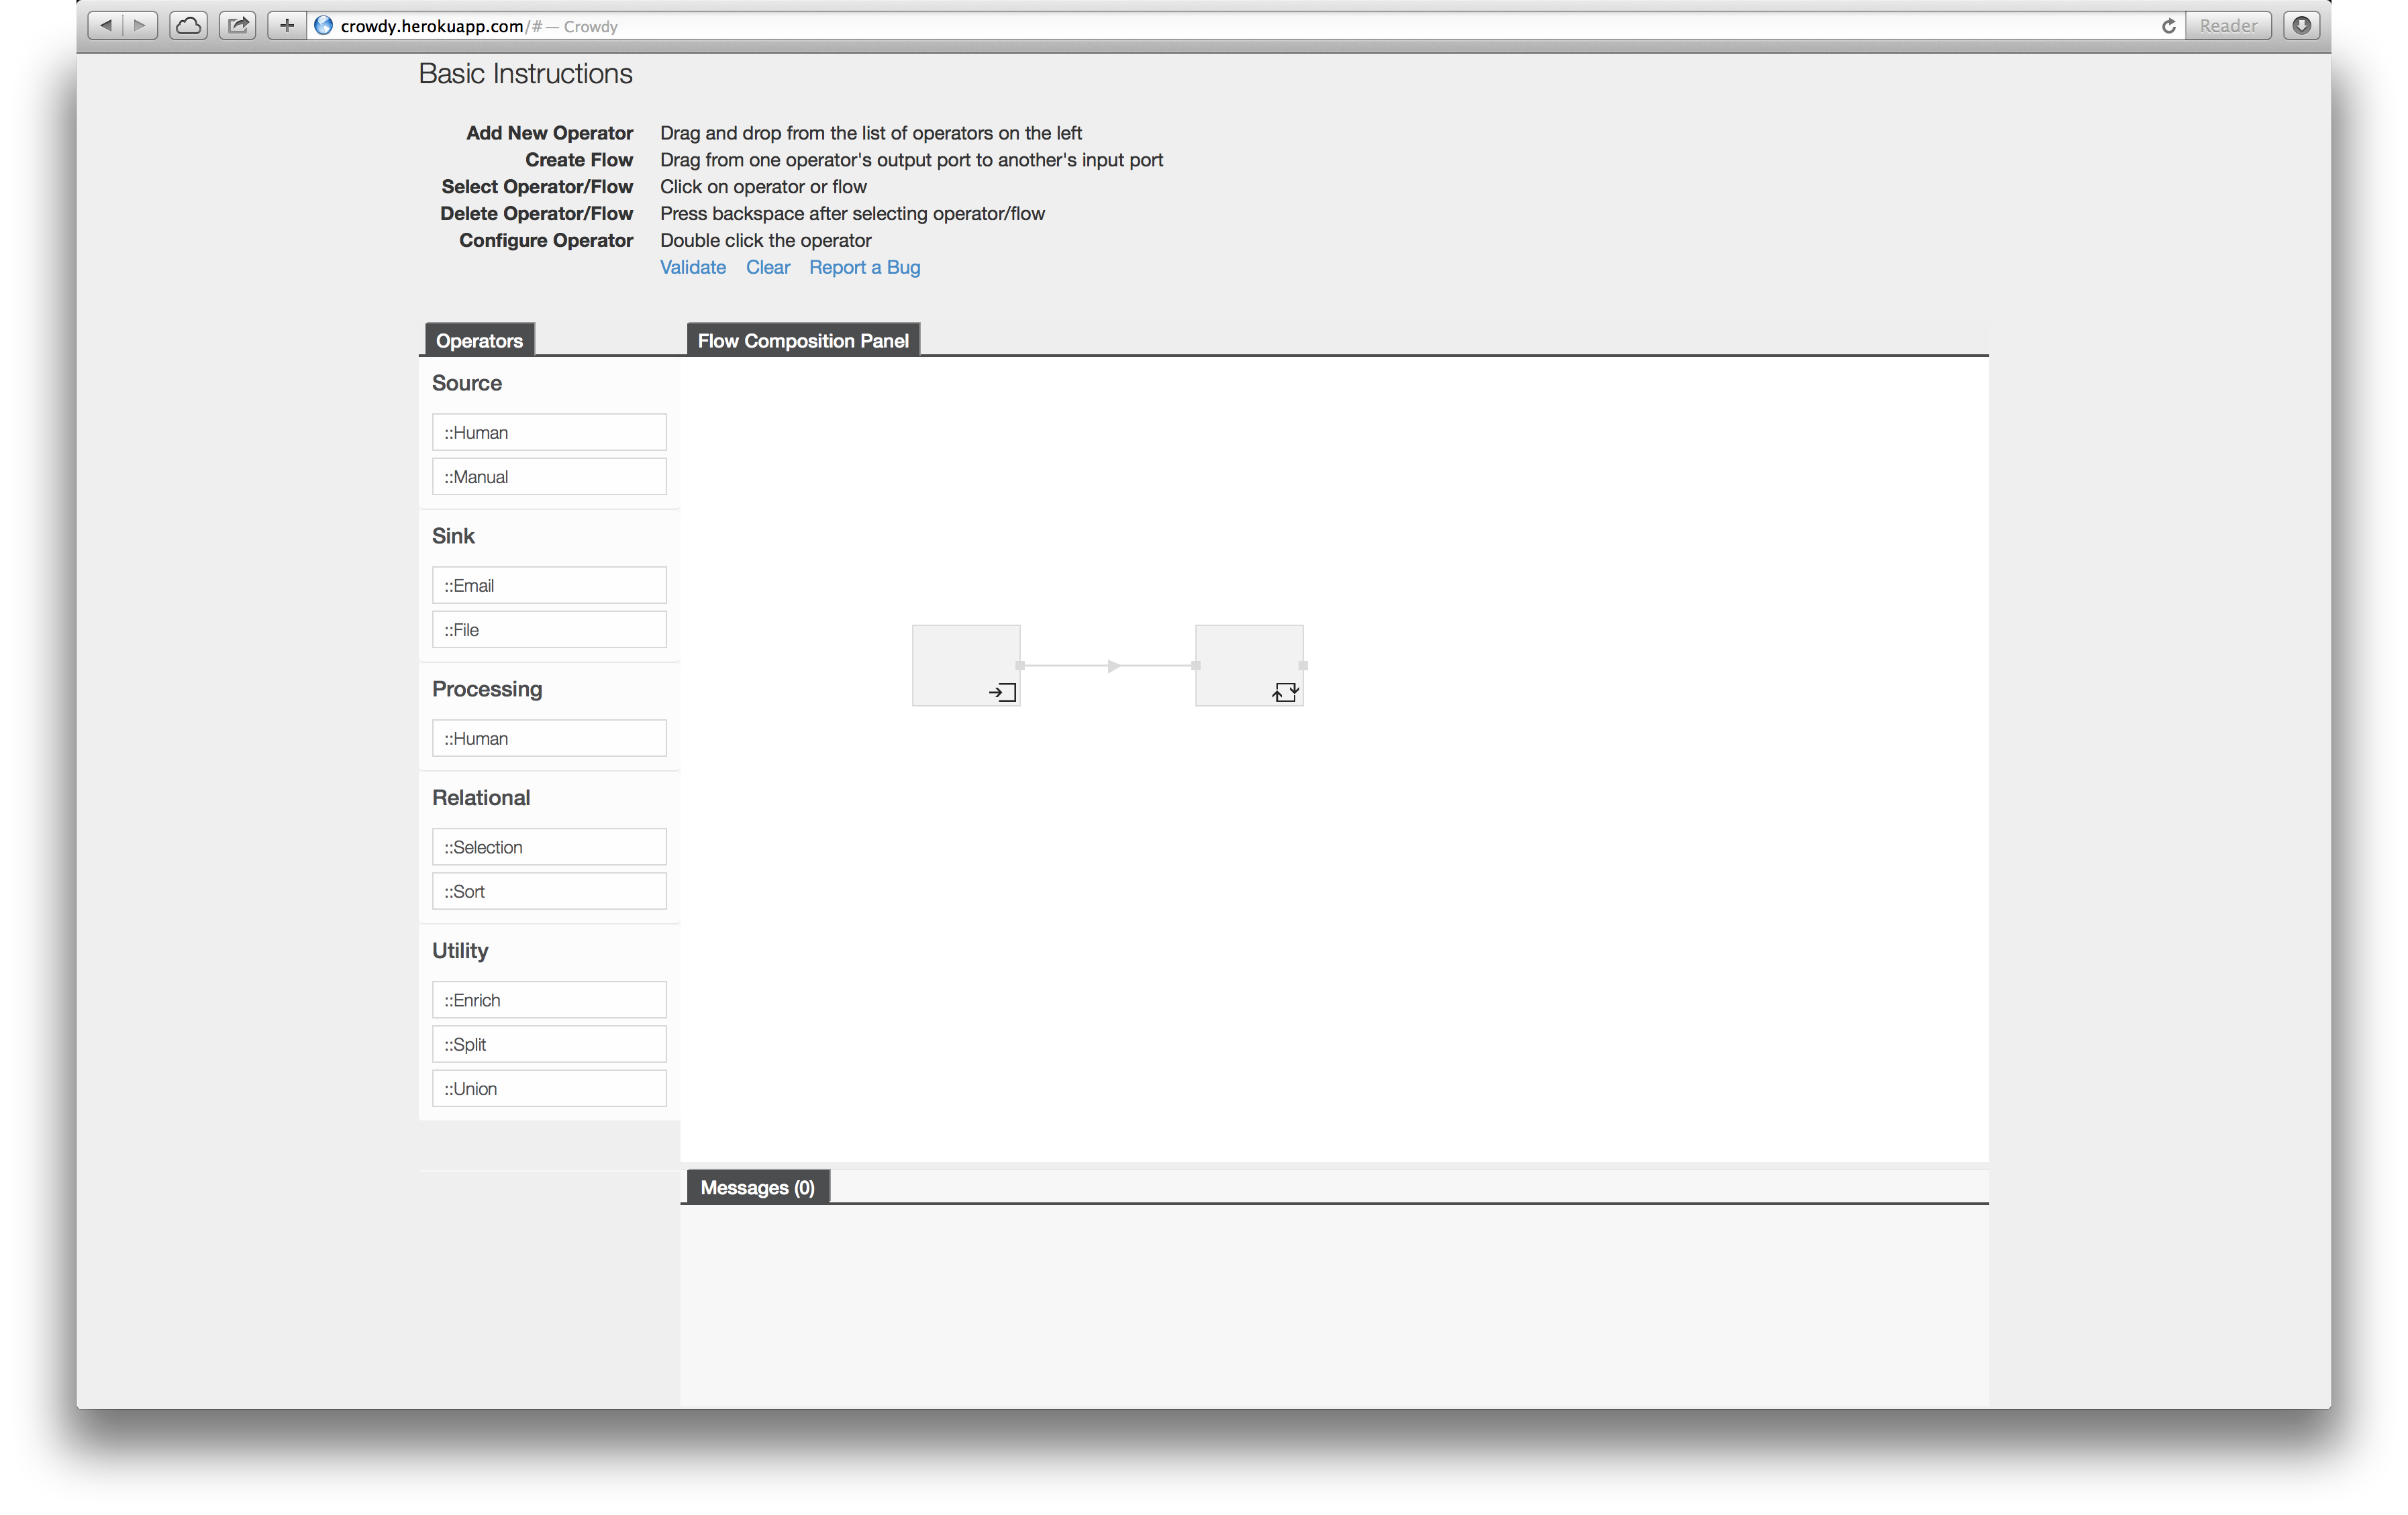
\includegraphics[width=0.9\textwidth]{figures/tool/panel5.png}
	\caption{Two operators connected via flow.}
	\label{fig:panel5}
\end{figure}

Figure~\ref{fig:panel6} shows the configuration window for 
\textit{human processing operator}, which is useful to create human tasks. 
Comparing this configuration with the previous 
one indicate the difference in the \textit{parameters} section. This section now presents 
the configuration specific to this operator. The fields are completed for the sake of 
demonstration and output specification is created. For instance, the data segment of 
the previous operator is available here to be able to create customizable questions 
under \textit{available segments} part. Those segments can be dragged and dropped 
to \textit{instructions}, \textit{question} and \textit{single/multiple choice} answer fields. 
Dropped segments can be easily deleted by pressing \textit{X} button on the right.

\begin{figure}[ht]
	\centering
	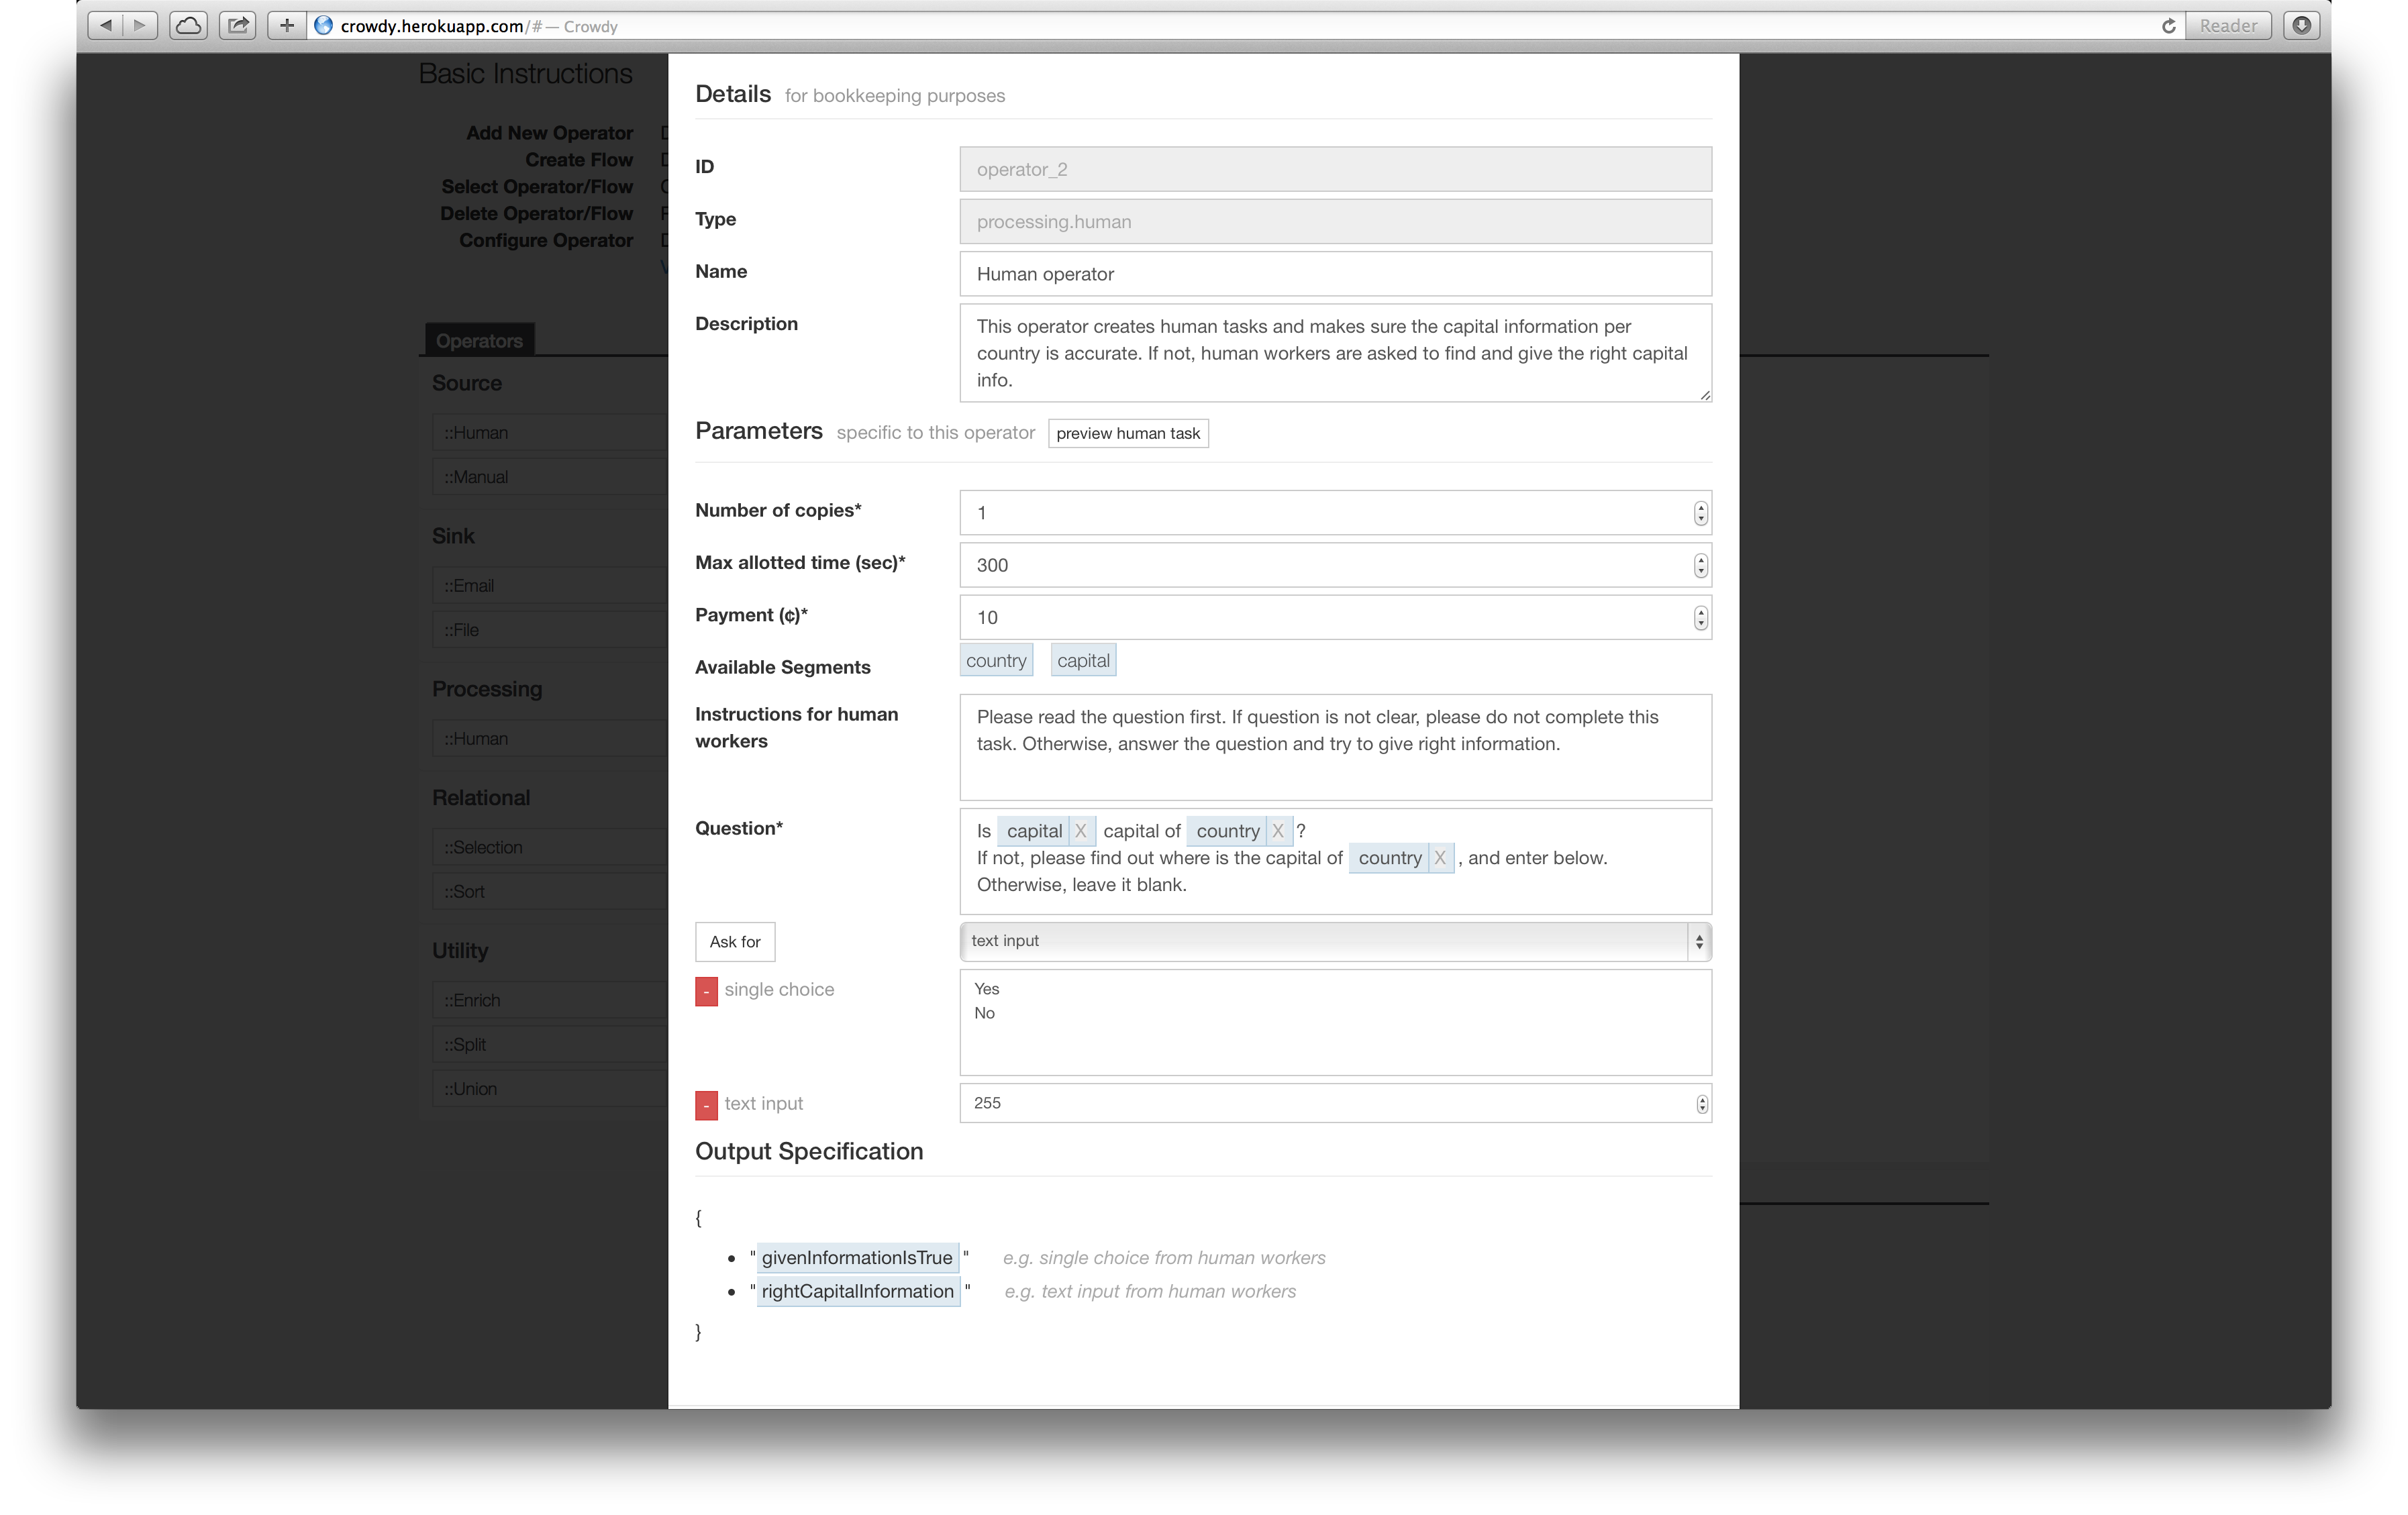
\includegraphics[width=0.9\textwidth]{figures/tool/panel6.png}
	\caption{Configuration window for human processing operator filled with sample information.}
	\label{fig:panel6}
\end{figure}

In addition, the human task that is configured in this operator can be previewed 
by clicking \textit{preview human task} button right near the \textit{parameters} 
section title. Figure~\ref{fig:panel7} shows the corresponding human task for 
that operator. The segments dropped in question field is presented using a different 
color. These will be automatically replaced with the segment value once 
information starts flowing from source to sink, which is when the application 
is executed.

\begin{figure}[ht]
	\centering
	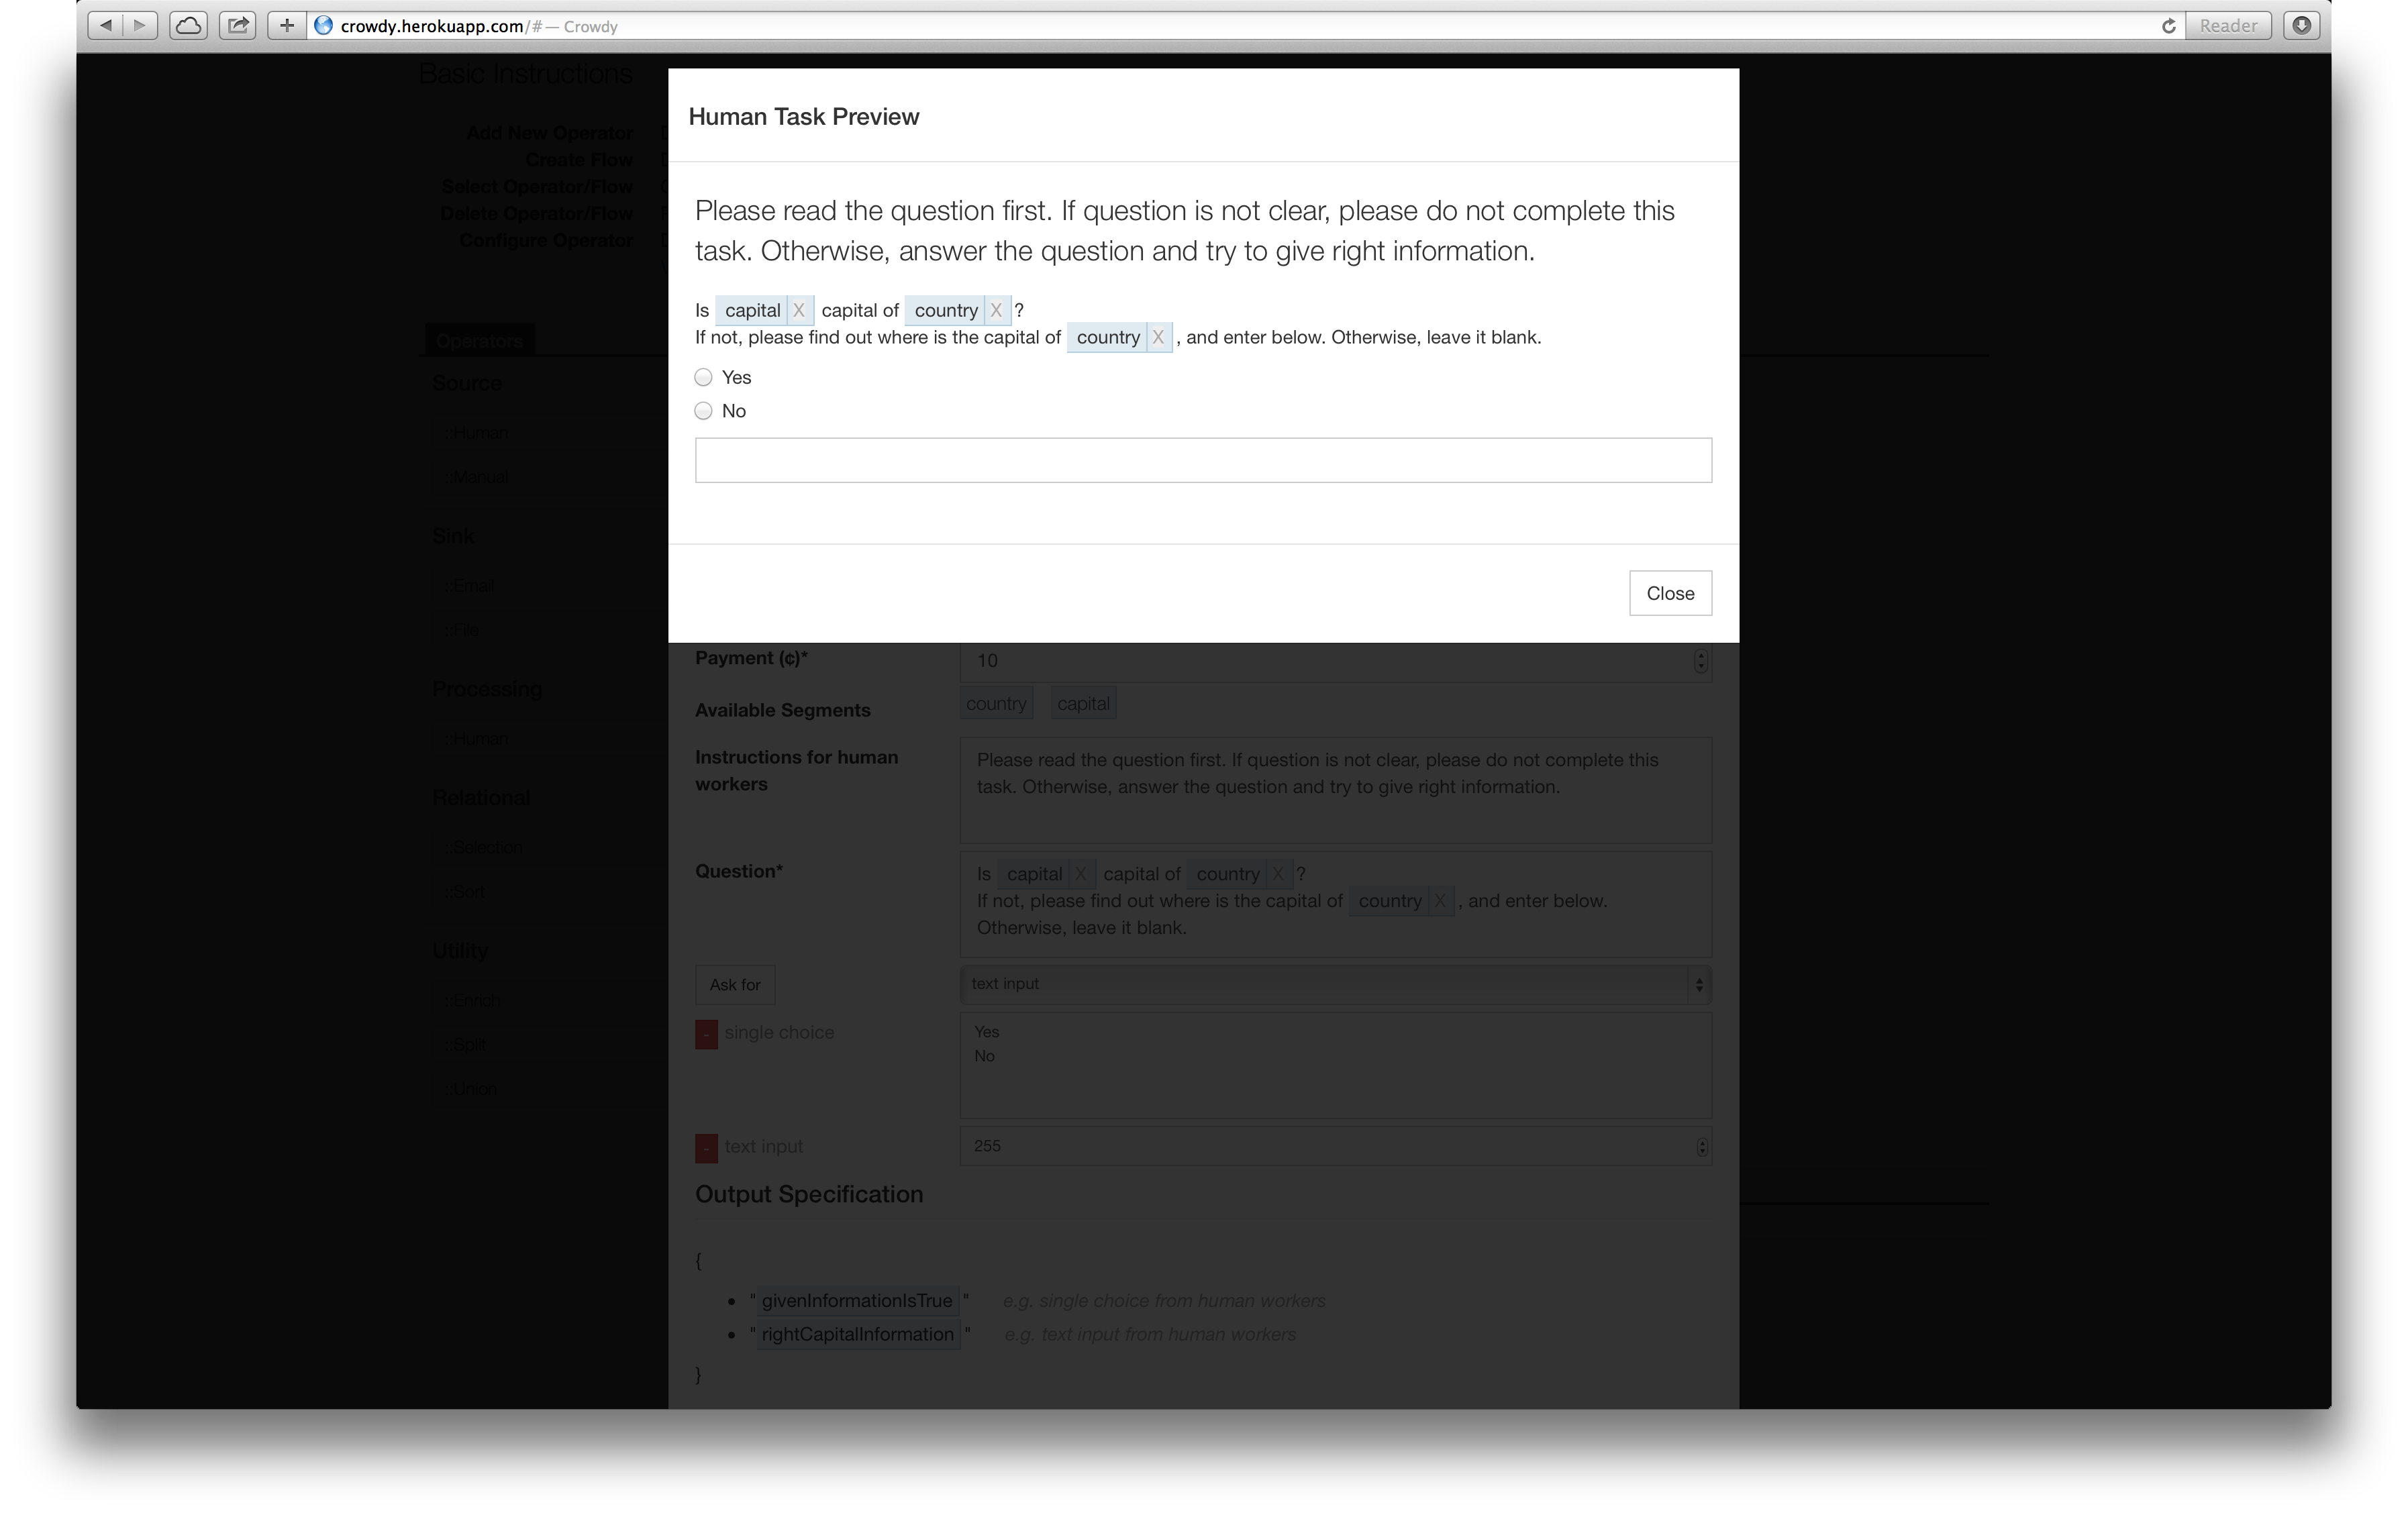
\includegraphics[width=0.9\textwidth]{figures/tool/panel7.png}
	\caption{Human task preview window for human processing operator.}
	\label{fig:panel7}
\end{figure}

Finally, a \textit{sink operator} is added and connected to 
\textit{human processing operator} as shown in Figure~\ref{fig:panel8}.

\begin{figure}[ht]
	\centering
	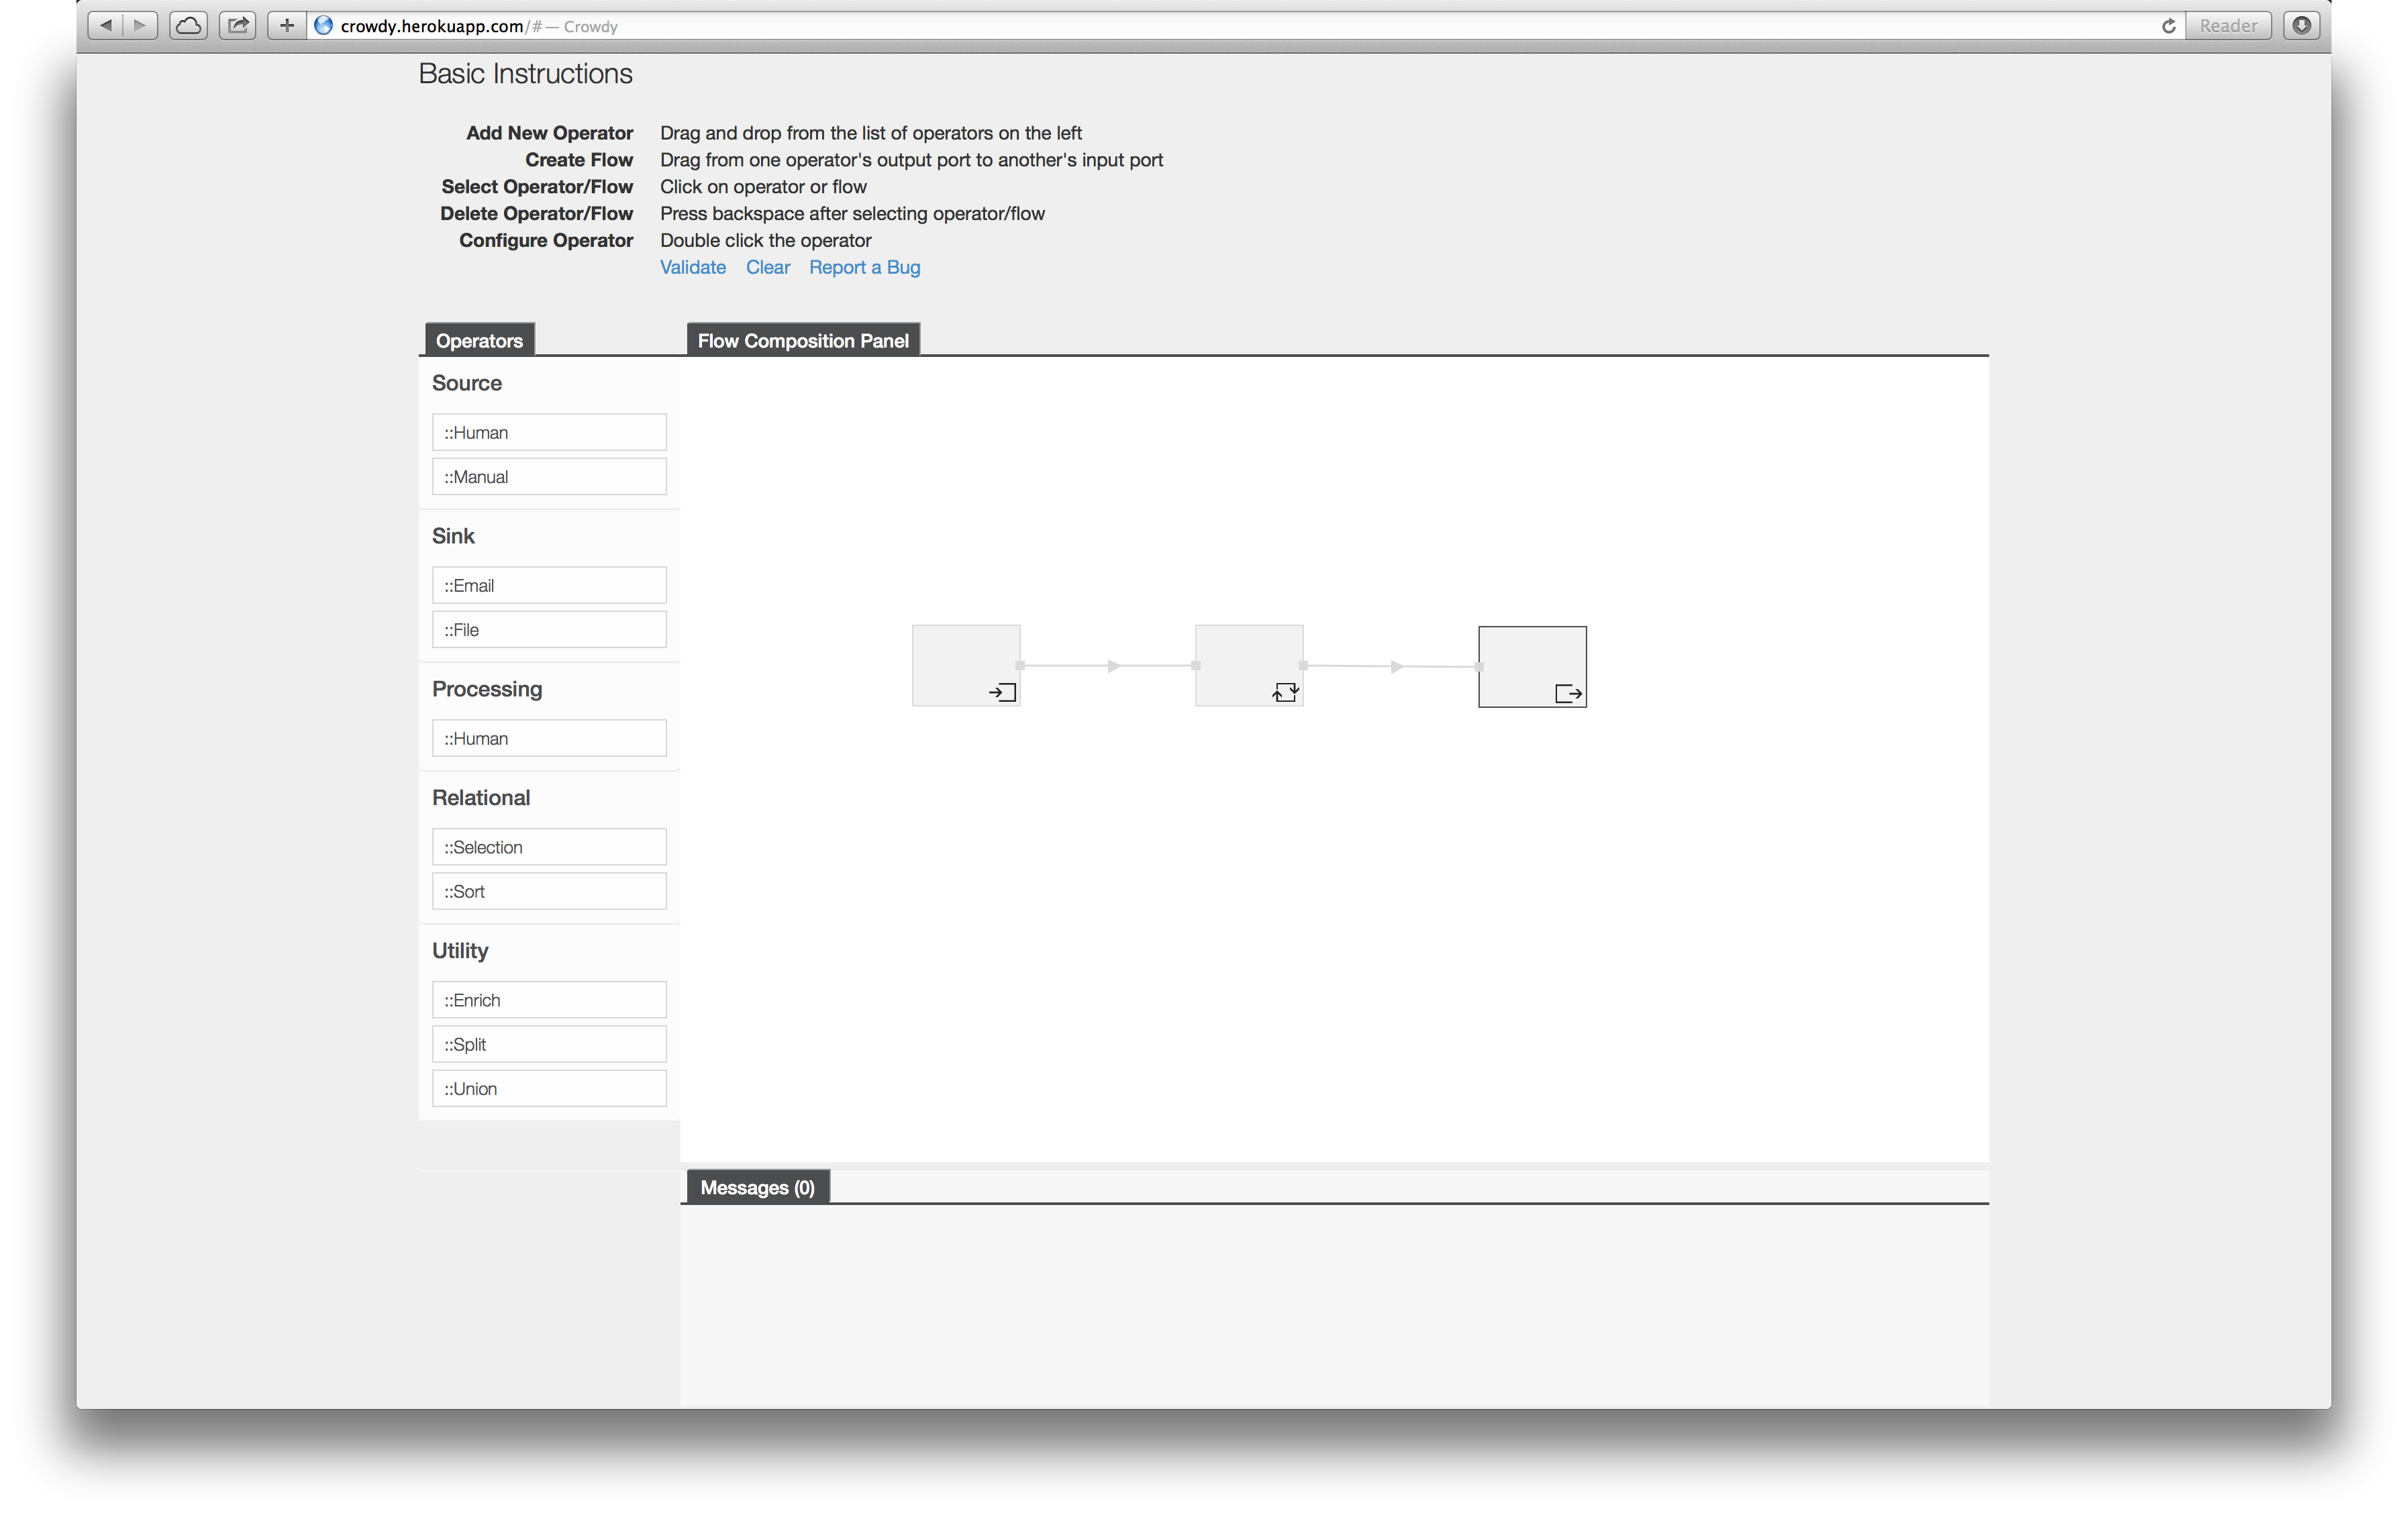
\includegraphics[width=0.9\textwidth]{figures/tool/panel8.png}
	\caption{A minimal application with source, processing and sink operators.}
	\label{fig:panel8}
\end{figure}

The configuration window (demonstrated in Figure~\ref{fig:panel9}) is intentionally 
left blank to show validation capabilities of $Crowdy$. Then, validation is 
initiated by clicking \textit{validate} link at the top of the flow composition window.

\begin{figure}[ht]
	\centering
	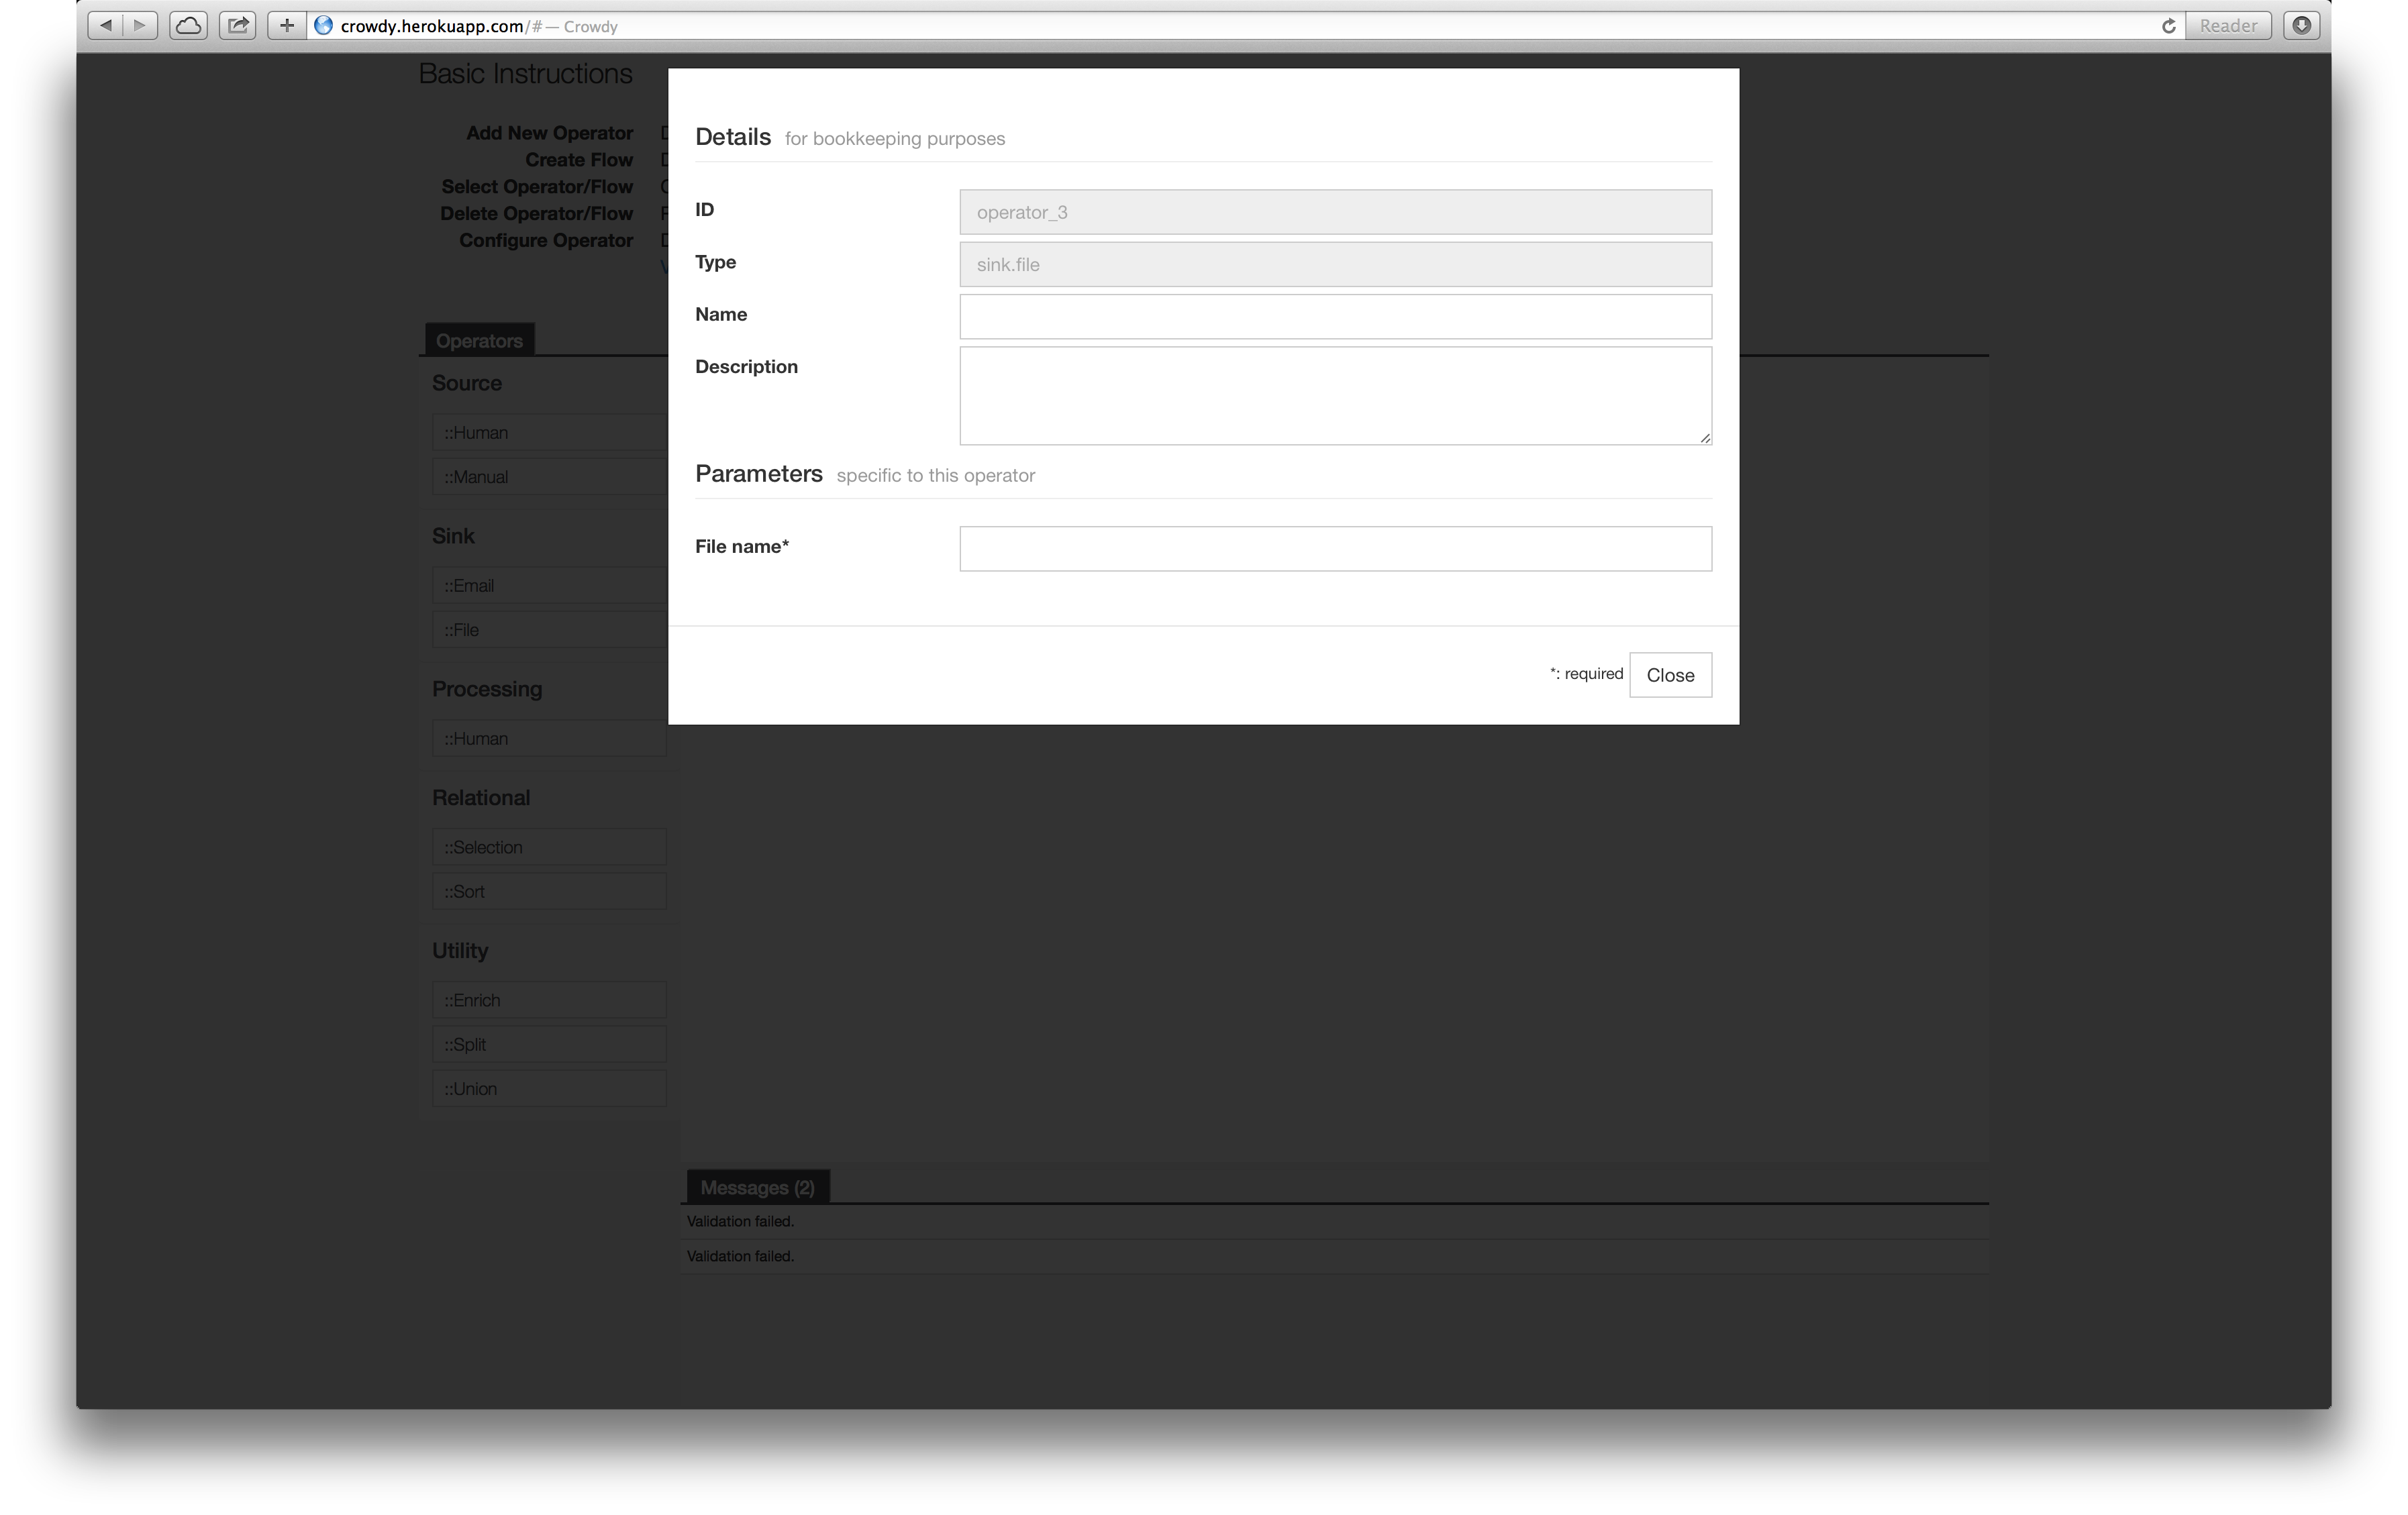
\includegraphics[width=0.9\textwidth]{figures/tool/panel9.png}
	\caption{Configuration window for sink operator.}
	\label{fig:panel9}
\end{figure}

The validation result is shown in Figure~\ref{fig:panel10}. The result lists all warnings 
and errors. An explanation per warning/error is given as well. Users are expected 
to resolve errors at least to complete validation and finally submit application for 
execution.

\begin{figure}[ht]
	\centering
	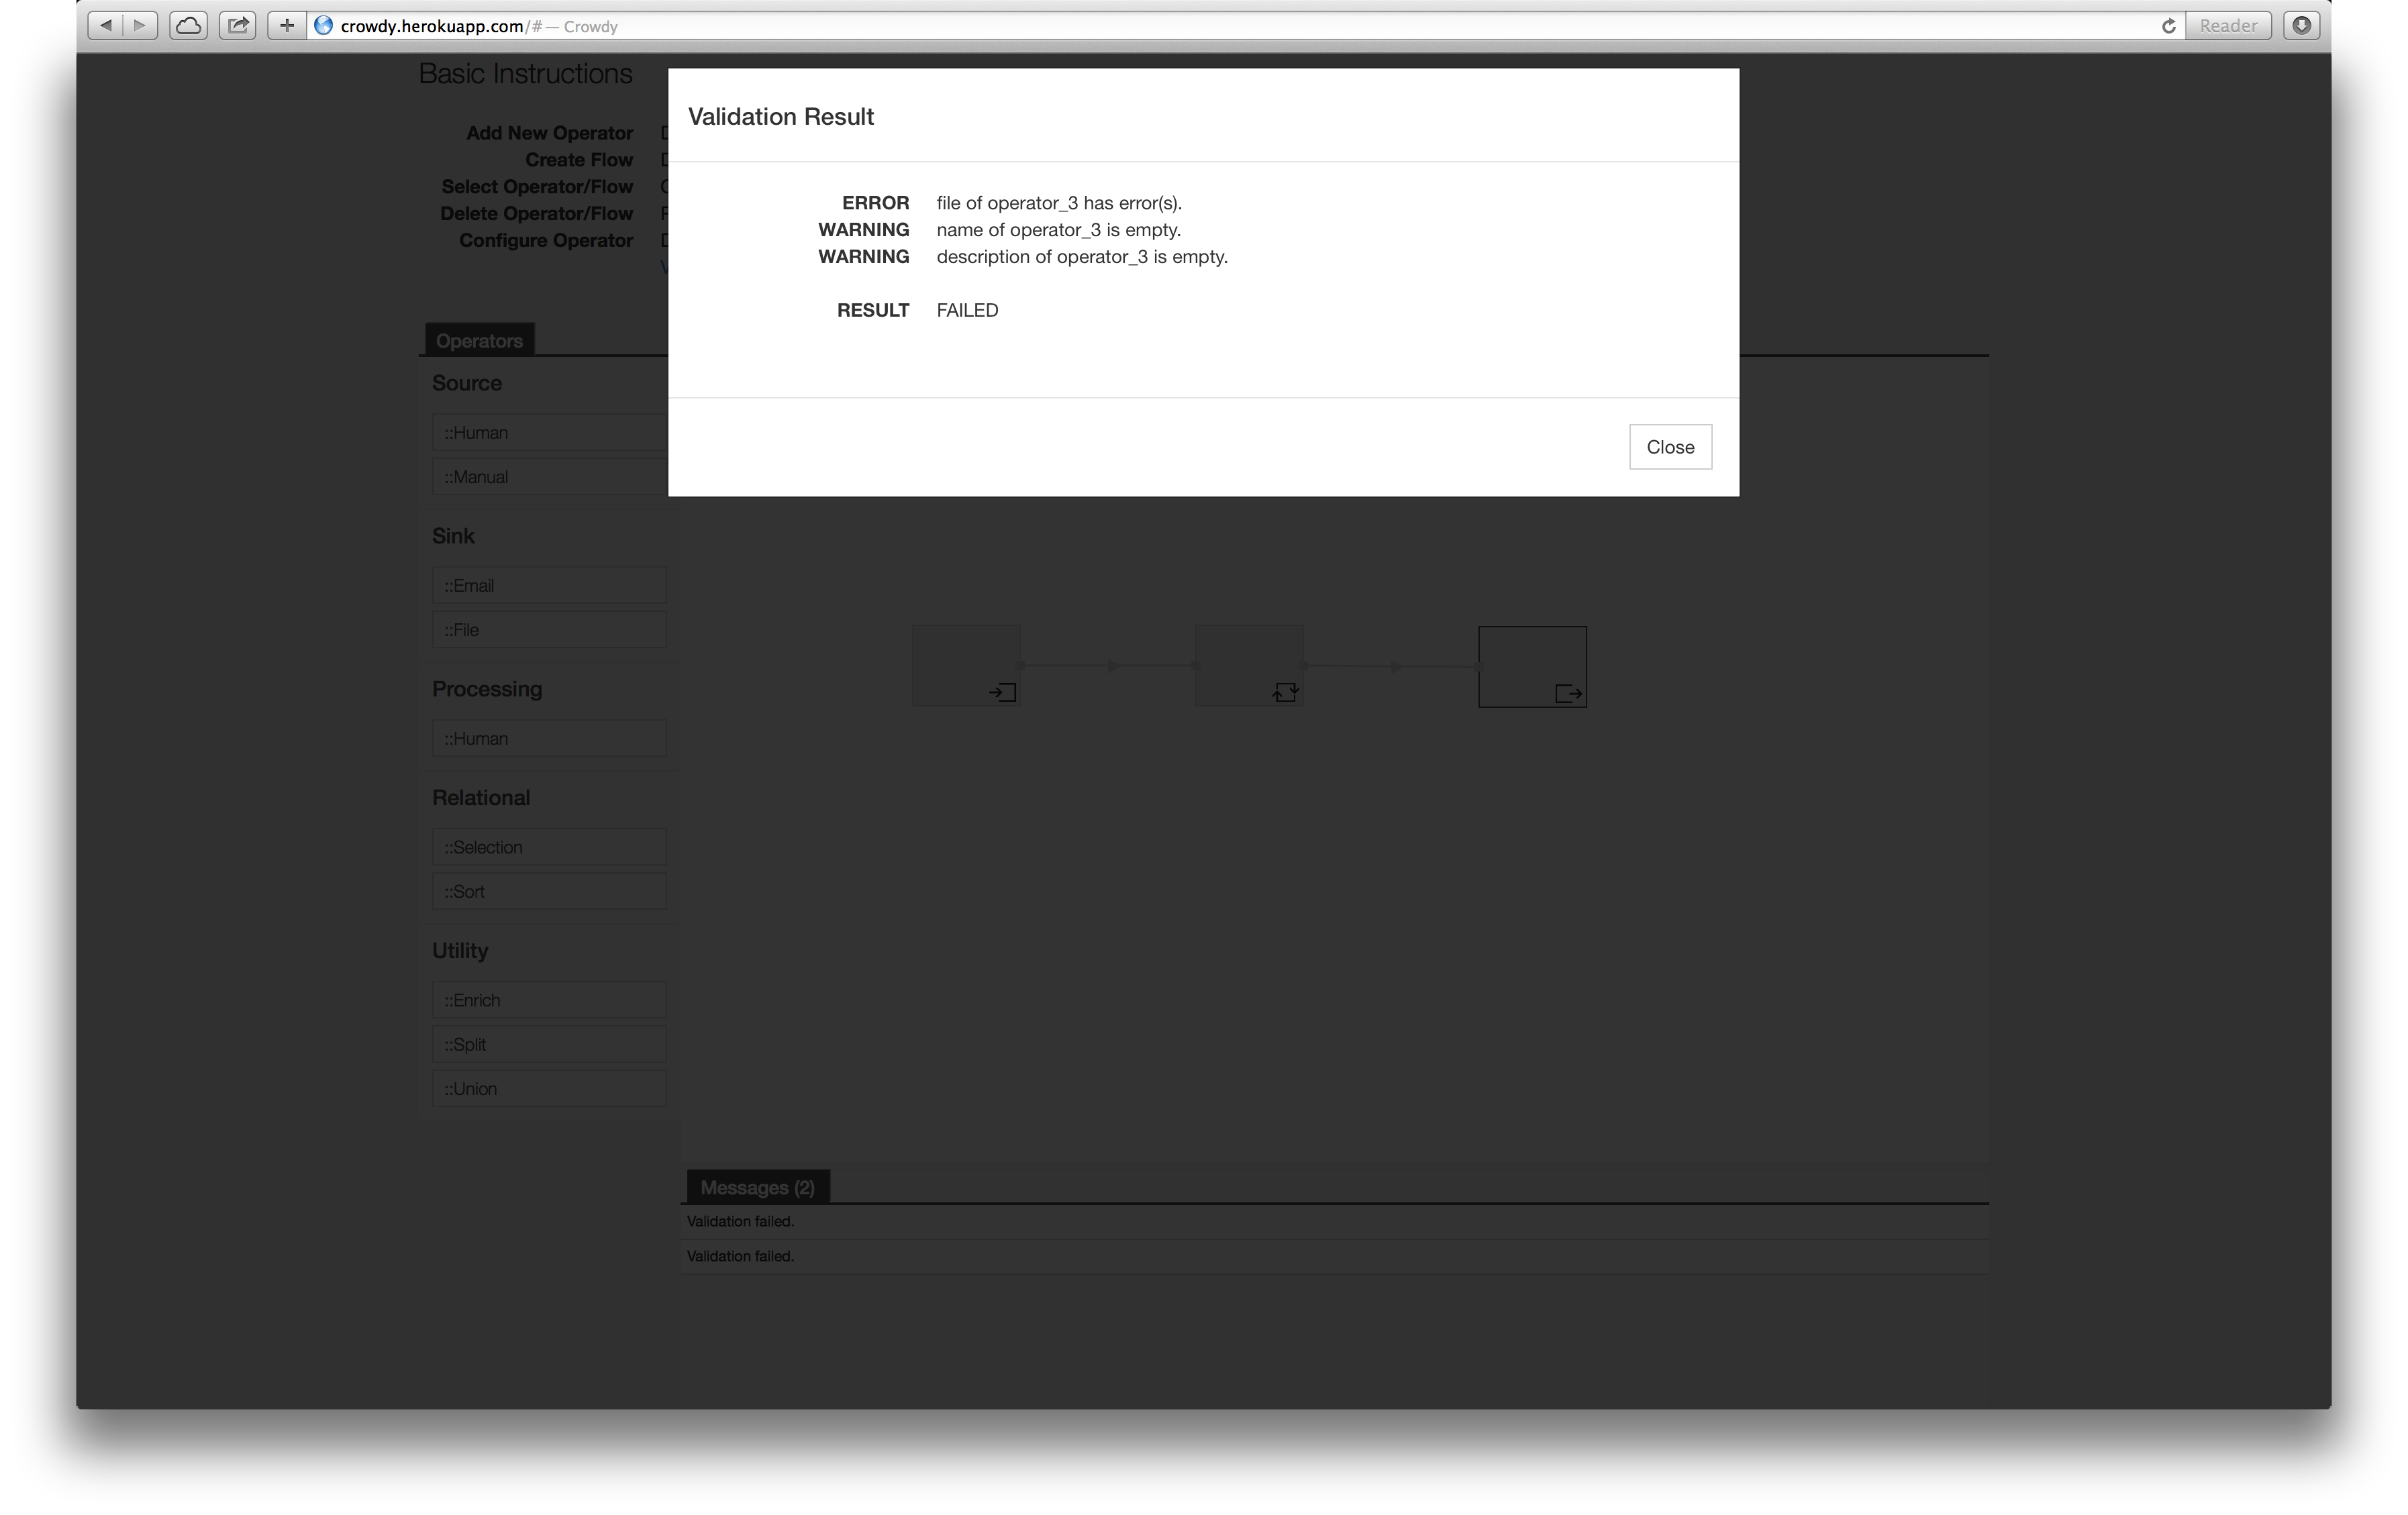
\includegraphics[width=0.9\textwidth]{figures/tool/panel10.png}
	\caption{Validation windows listing warnings and errors.}
	\label{fig:panel10}
\end{figure}

When we open the configuration window for \textit{sink operator}, which is the source 
of validation problems, the problematic fields are marked with yellow for warning and 
red for error (see Figure~\ref{fig:panel11}). Since \textit{file name} is required and it is 
left empty, it caused an error during validation.

\begin{figure}[ht]
	\centering
	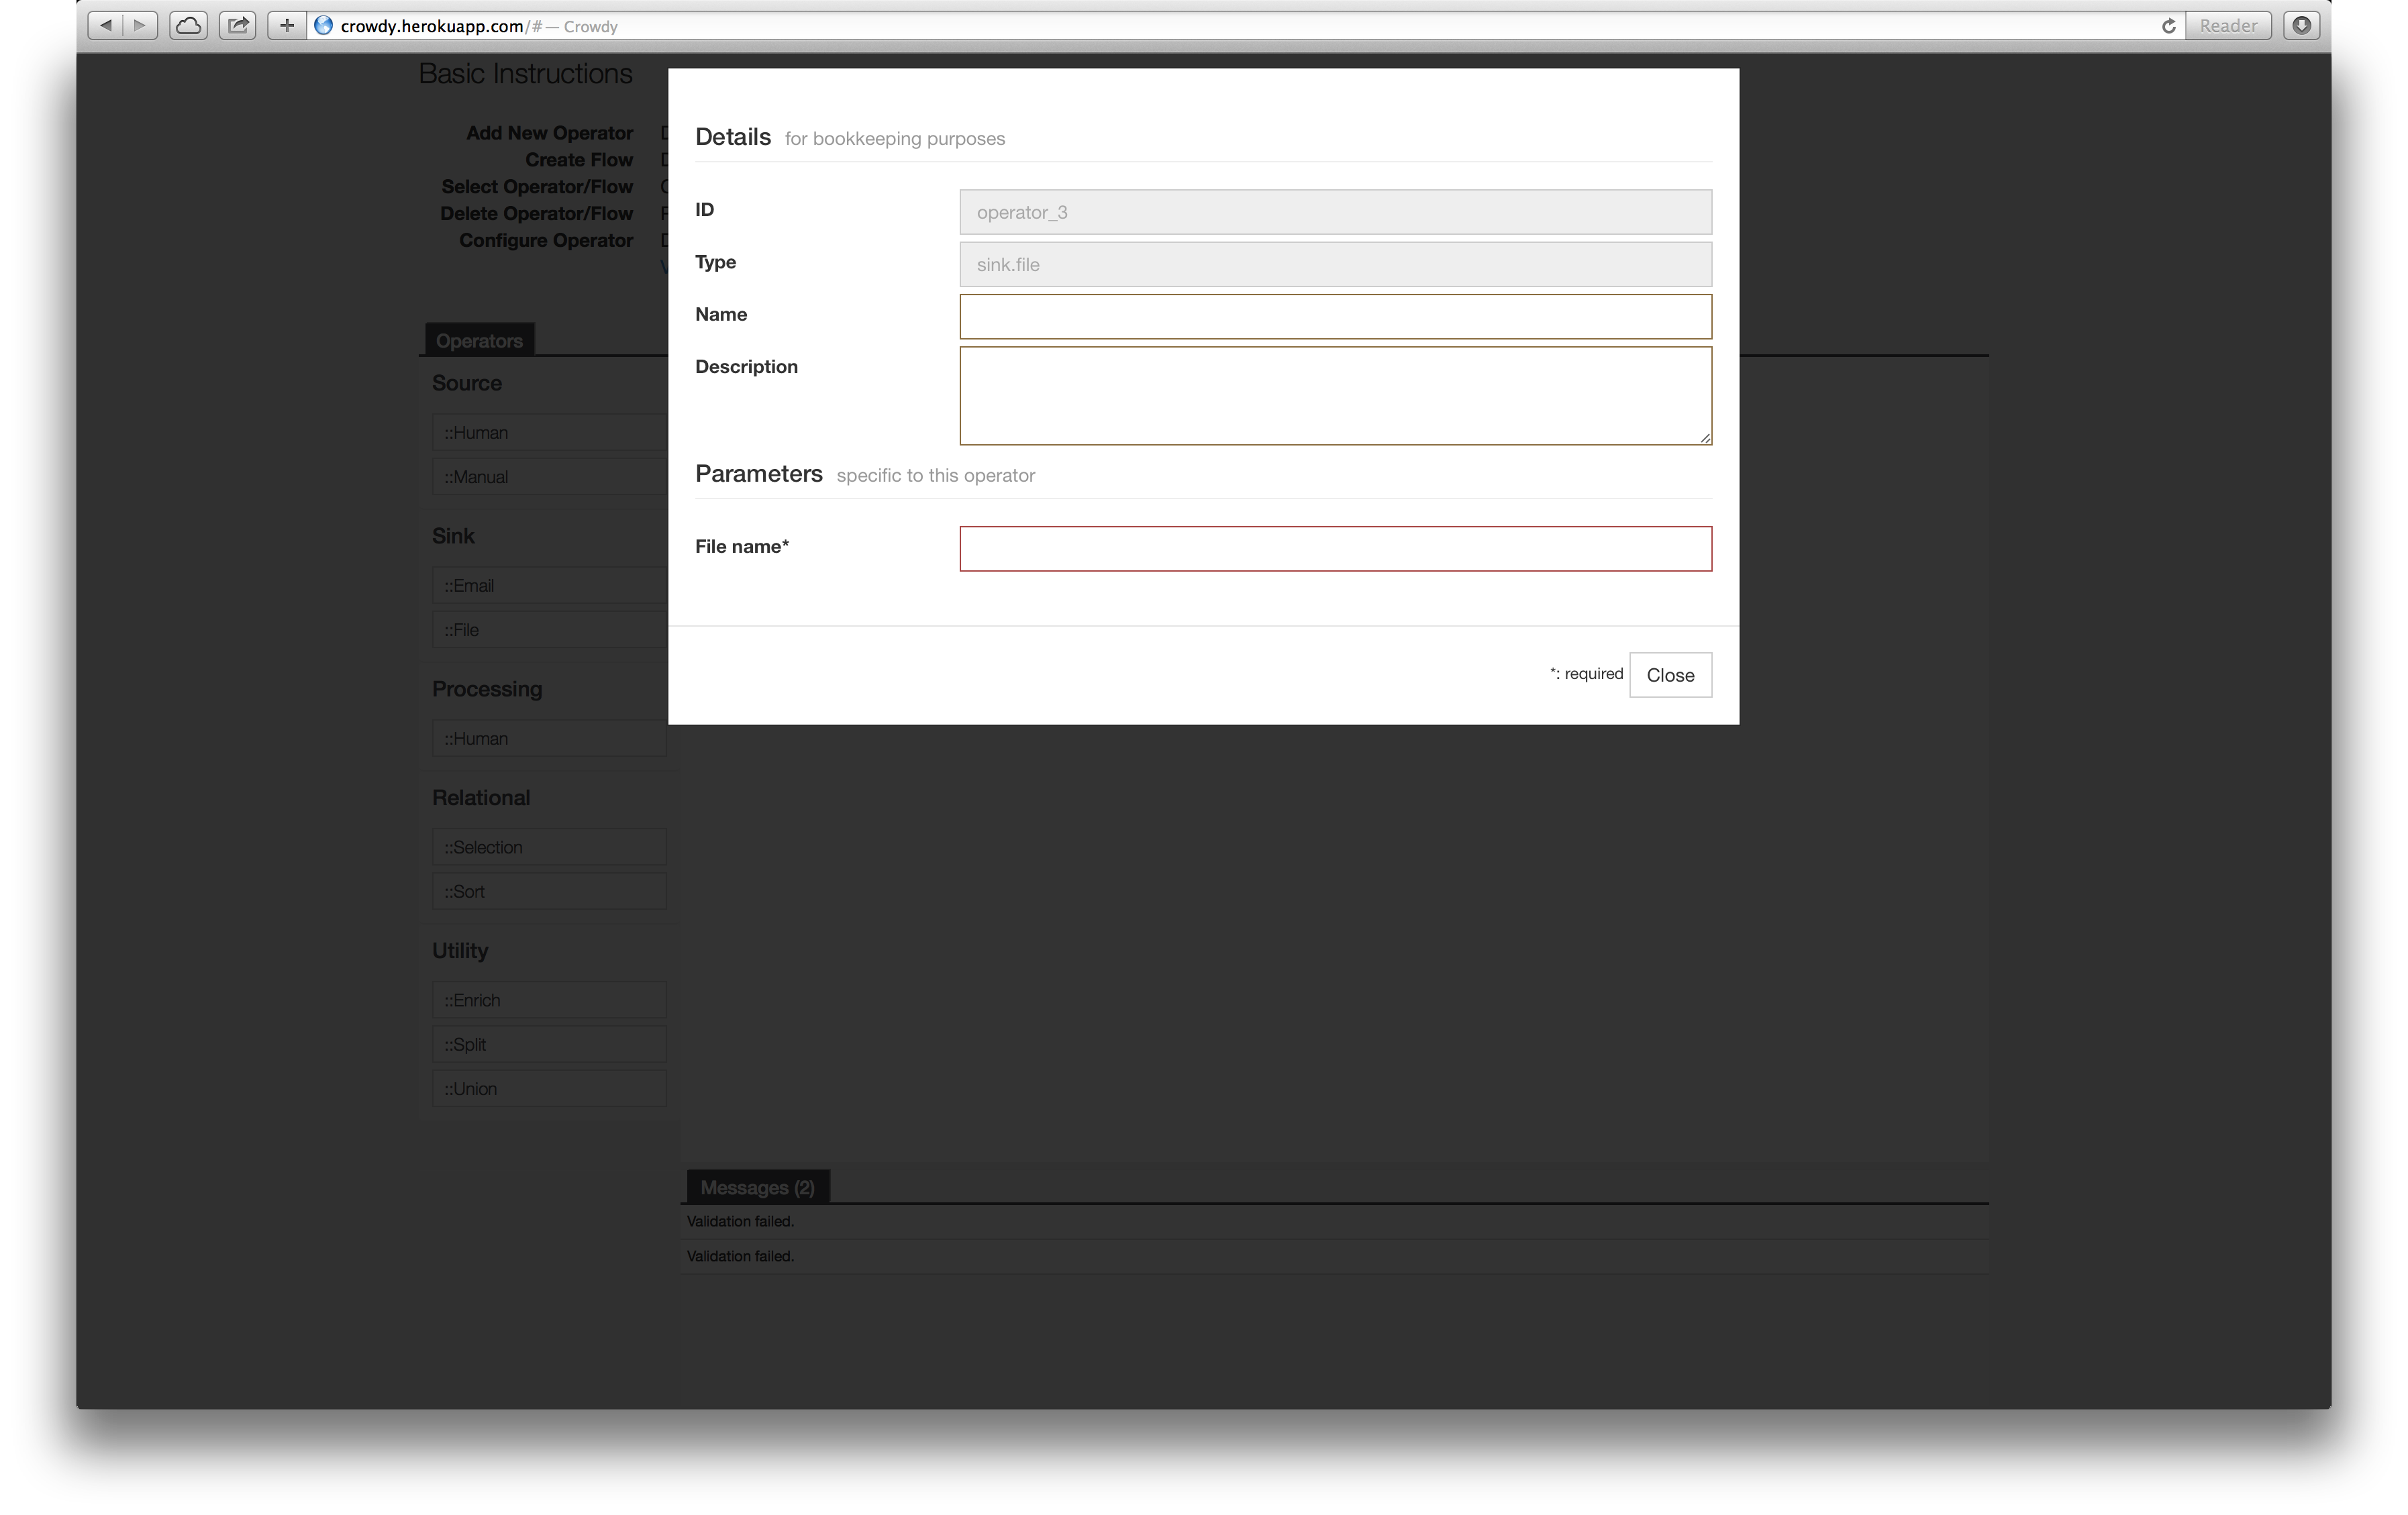
\includegraphics[width=0.9\textwidth]{figures/tool/panel11.png}
	\caption{Configuration window for sink operator after validation.}
	\label{fig:panel11}
\end{figure}

At least the errors should be resolved for validation to succeed. Once validation goes 
through application can be submitted for execution via the link appearing on right bottom 
of validation window demonstrated in Figure~\ref{fig:panel12}. After application is 
submitted, the processes are created and appropriate resources are allocated to solve 
the problem and find the result. In this specific example, results are expected to be 
written into a file.

\begin{figure}[ht]
	\centering
	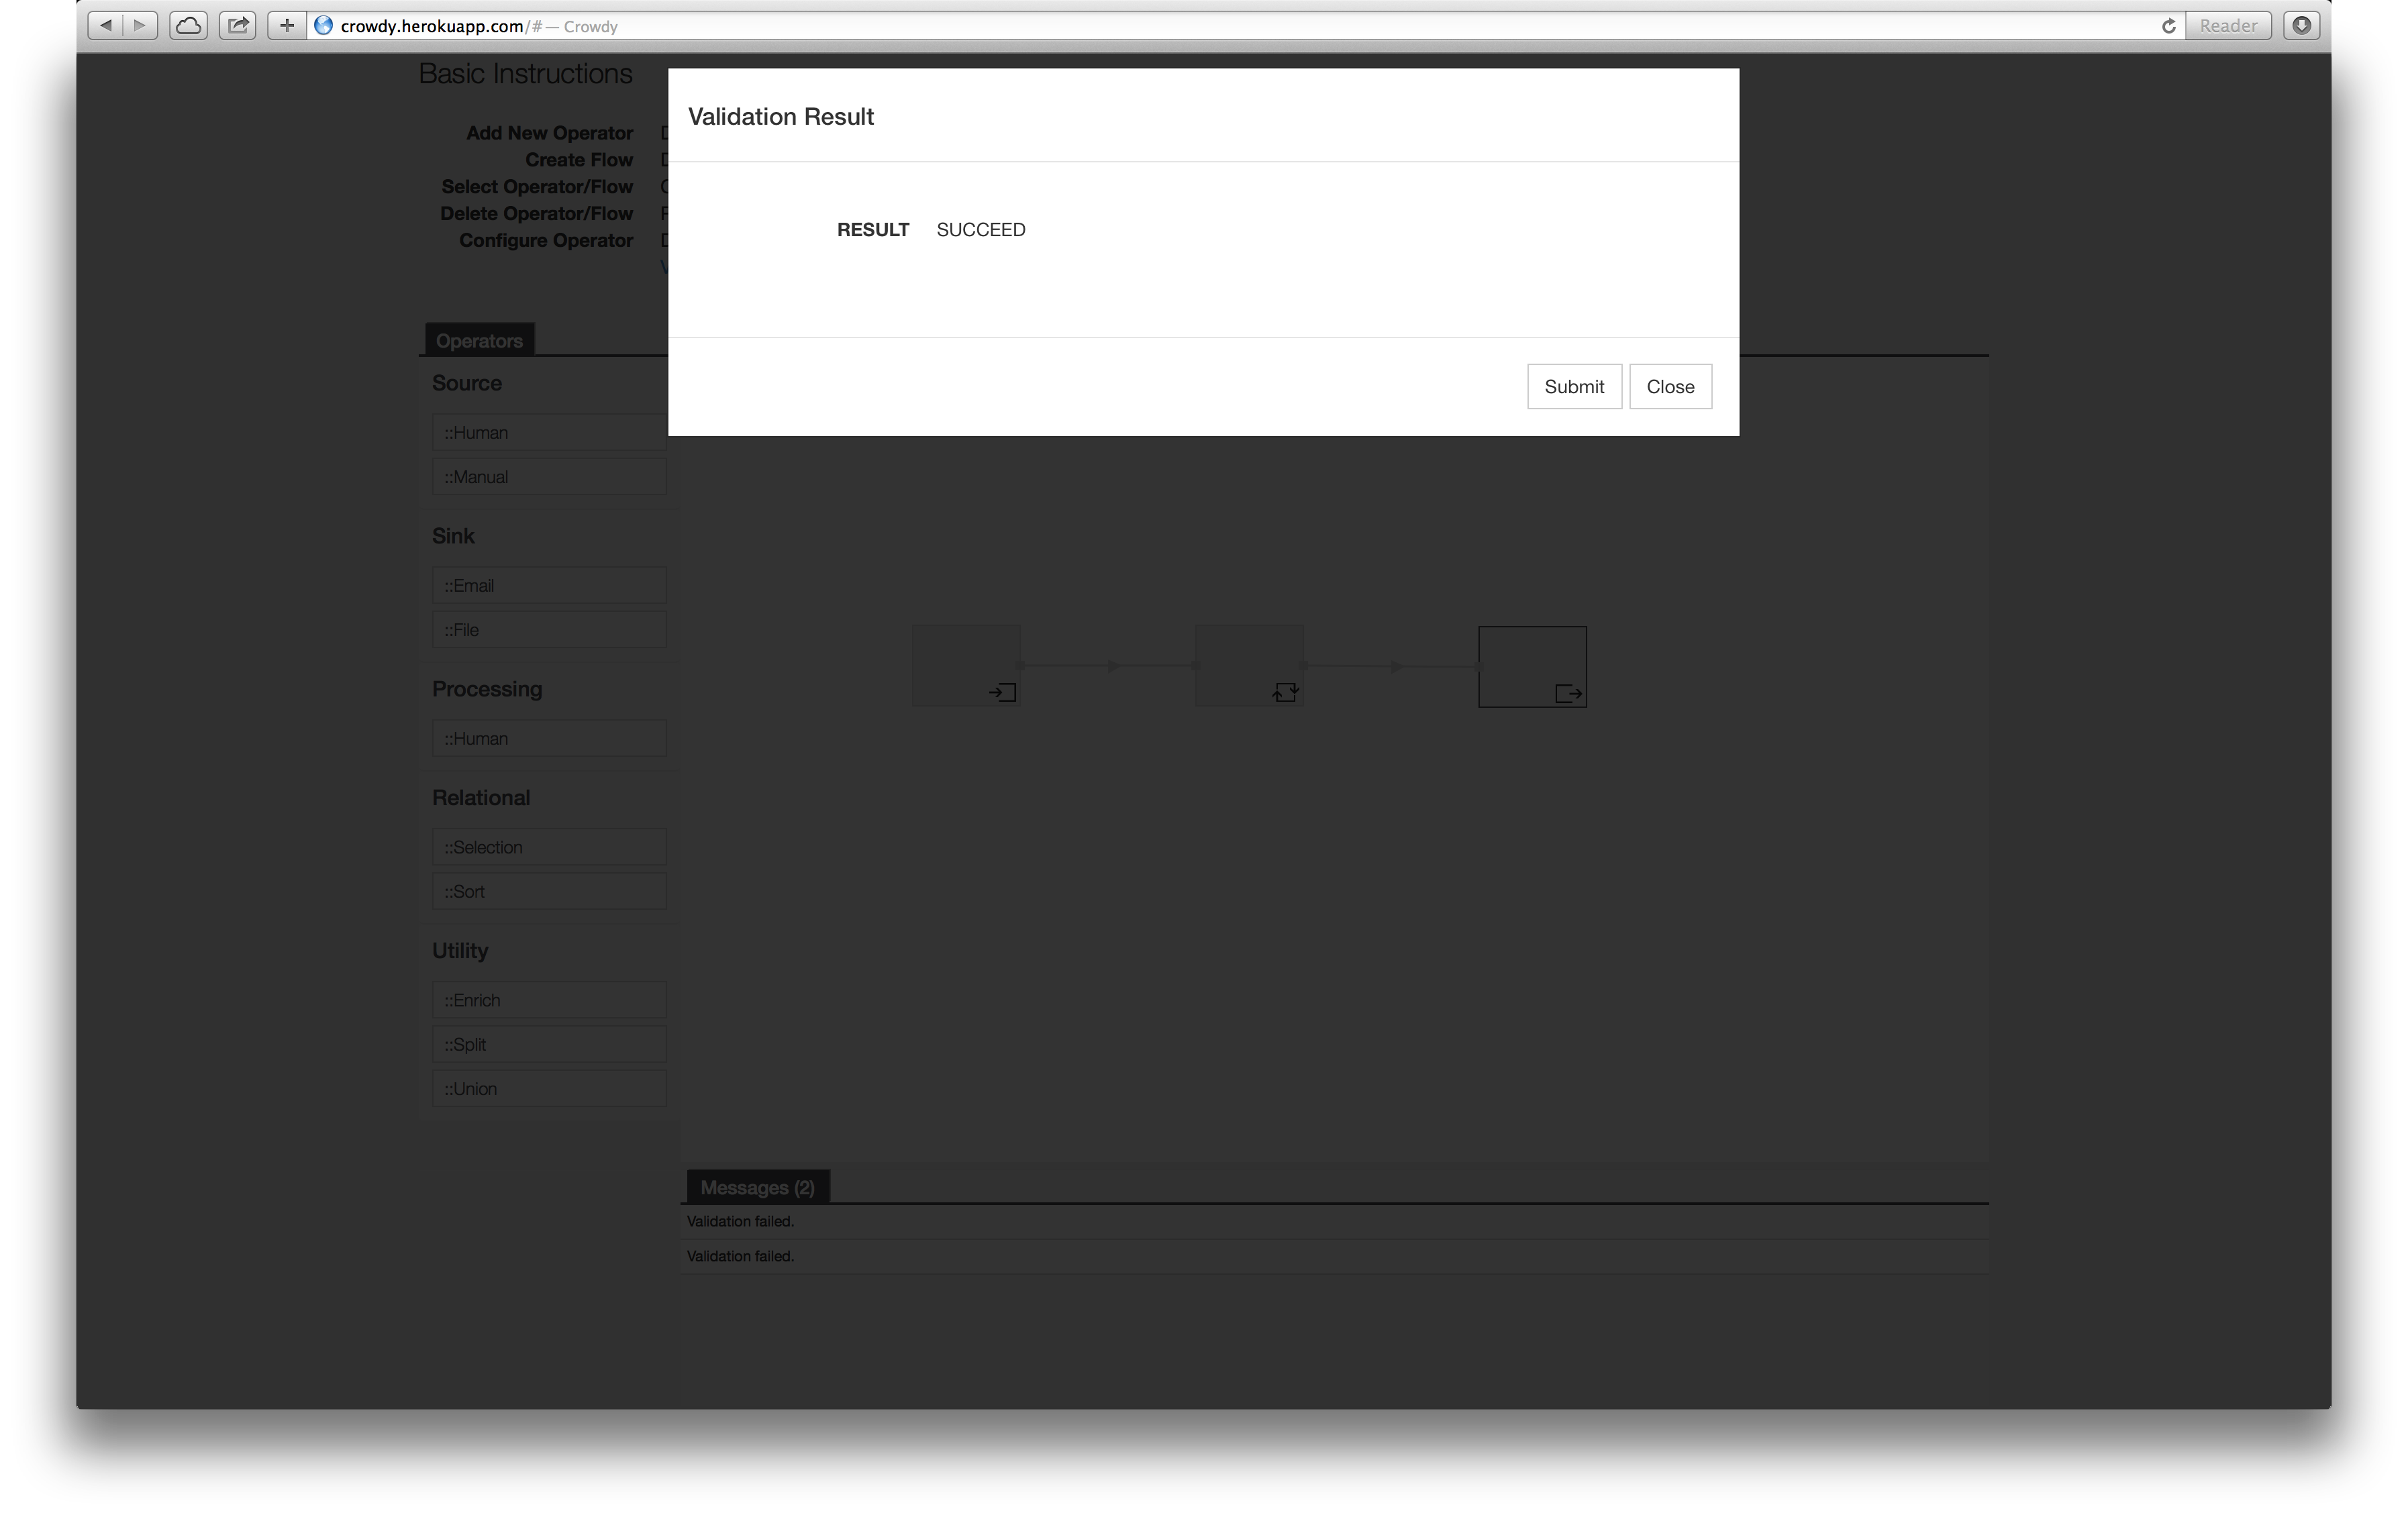
\includegraphics[width=0.9\textwidth]{figures/tool/panel12.png}
	\caption{Successful validation window with submit link.}
	\label{fig:panel12}
\end{figure}

Finally, Figure~\ref{fig:panel13} shows the window to report a bug. Bugs can be 
reported using this window. While custom messages can be given, the tool itself 
gather particular logs for that session to create an application.

\begin{figure}[ht]
	\centering
	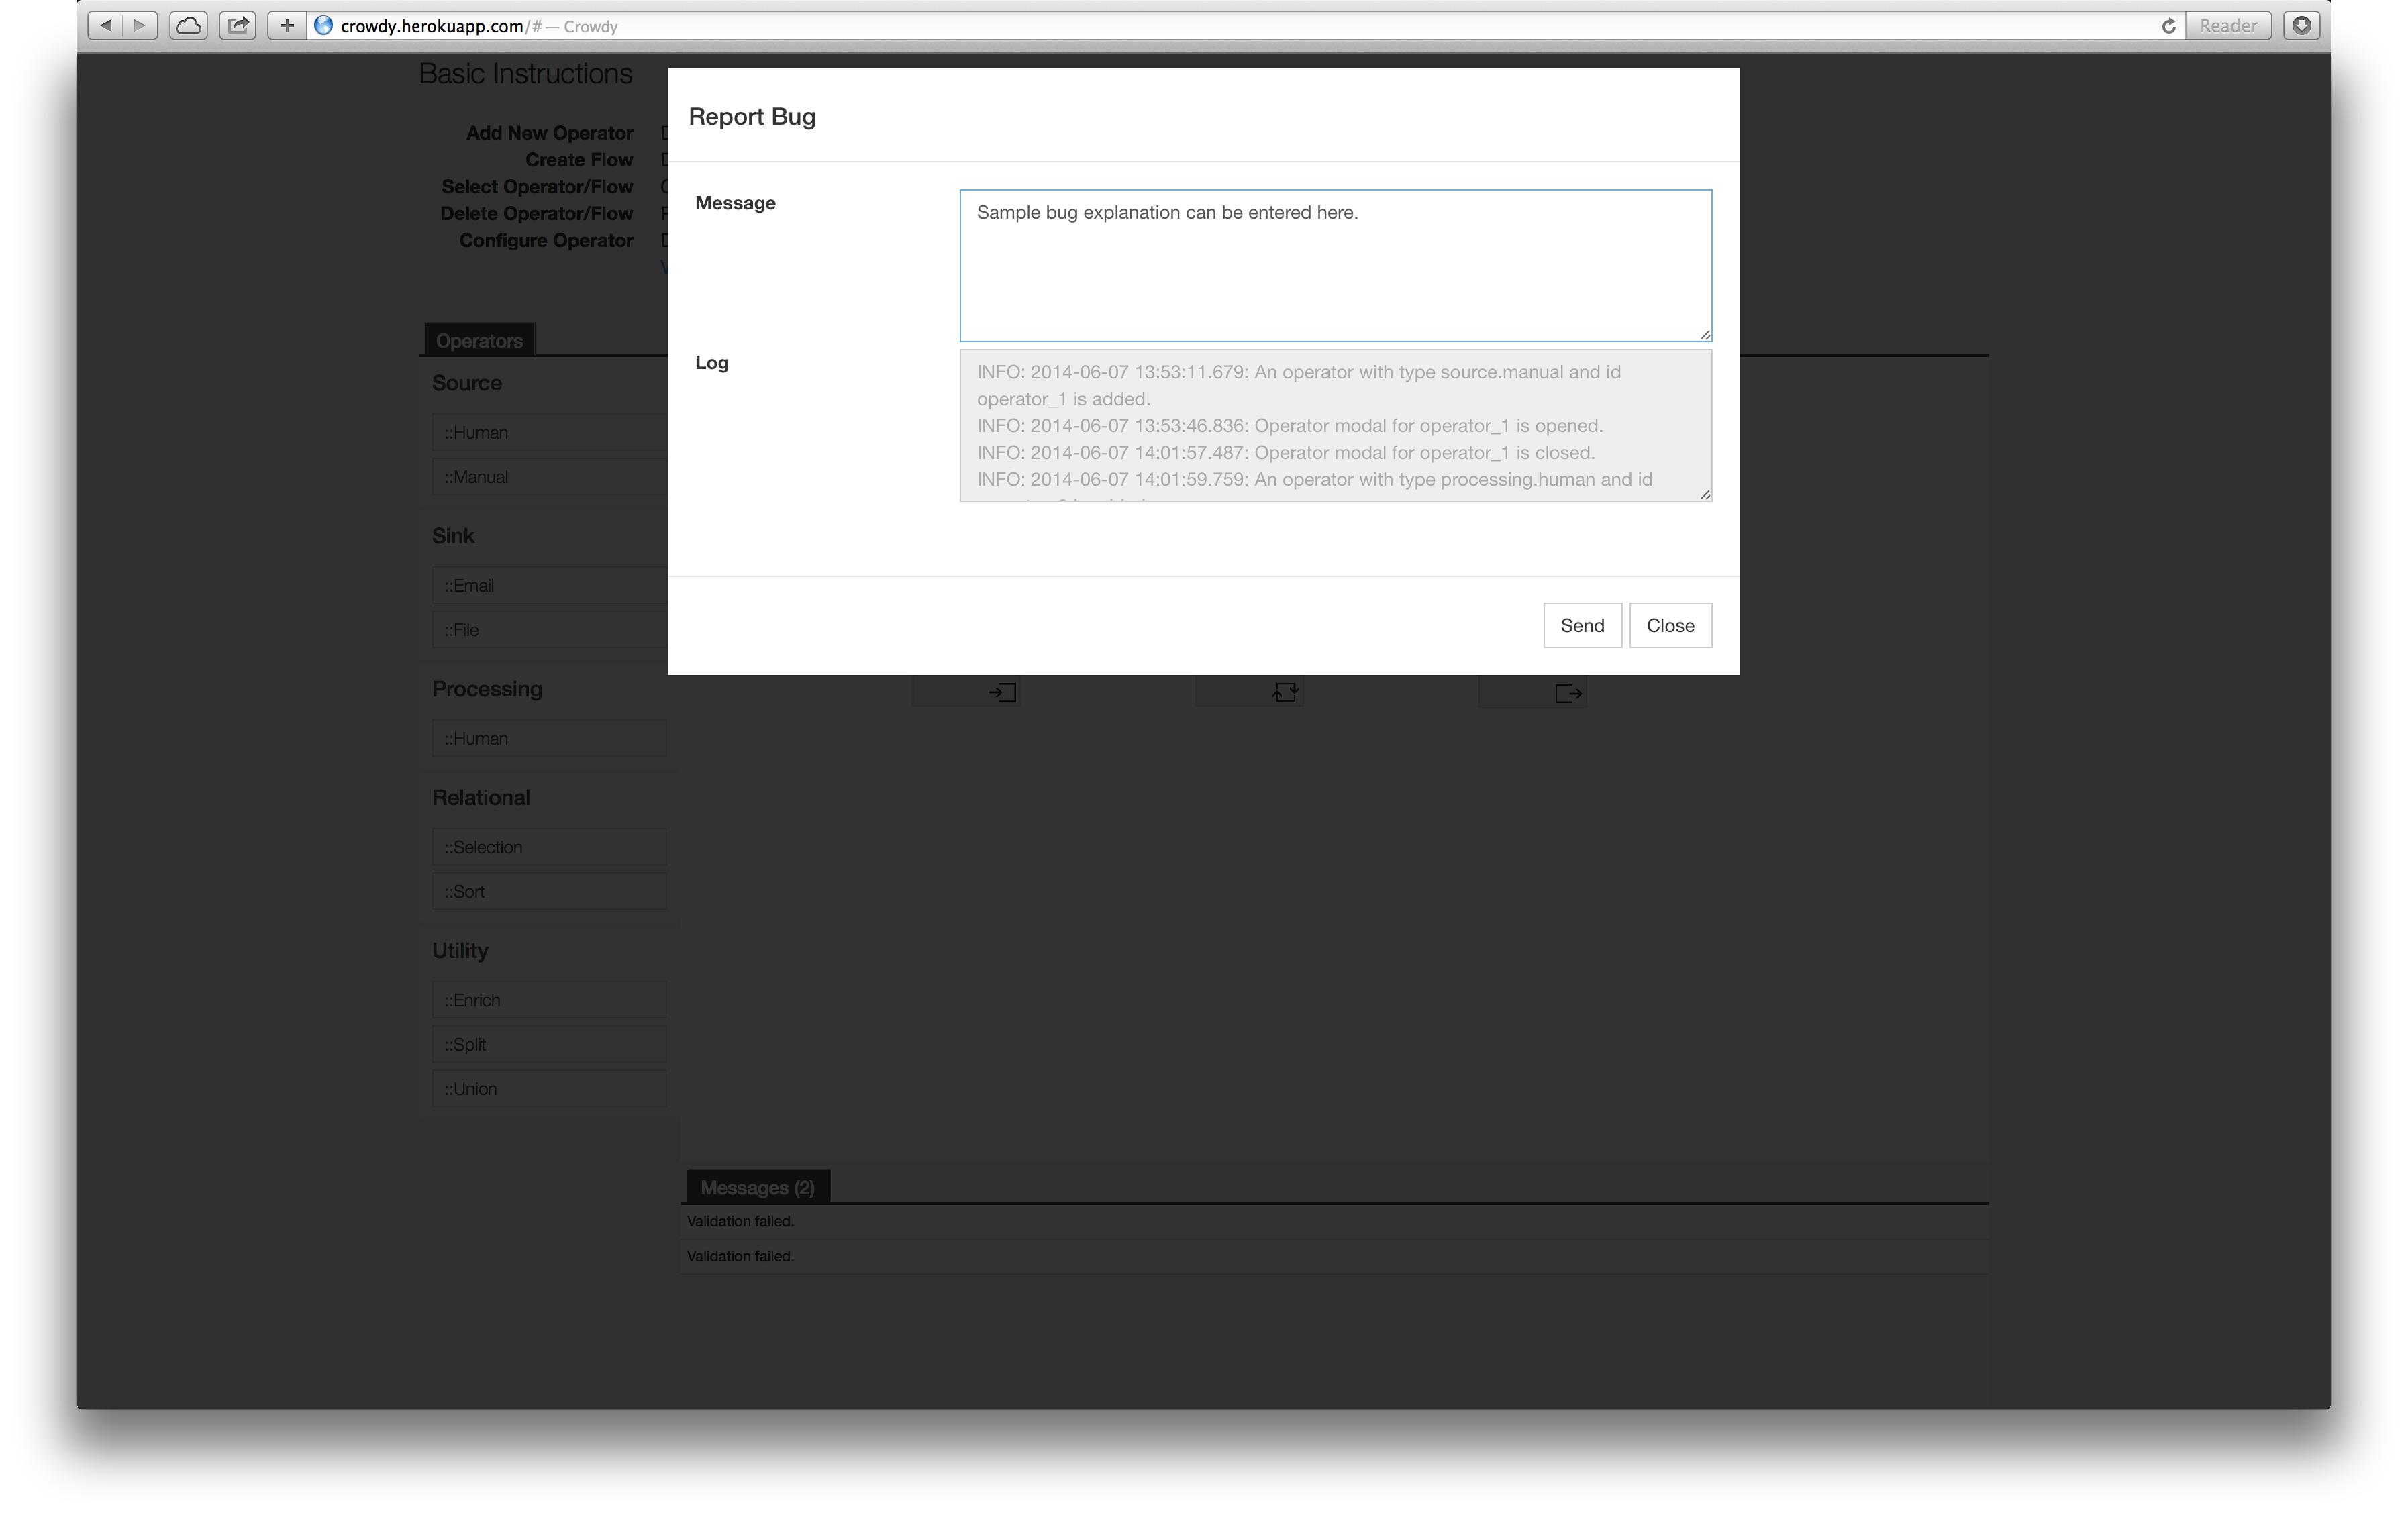
\includegraphics[width=0.9\textwidth]{figures/tool/panel13.png}
	\caption{Window to report a bug.}
	\label{fig:panel13}
\end{figure}
